%% 使用 njuthesis 文档类生成南京大学学位论文的示例文档
%%
%% 作者:胡海星,starfish (at) gmail (dot) com
%% 项目主页: http://haixing-hu.github.io/nju-thesis/
%%
%% 本样例文档中用到了吕琦同学的博士论文的提高和部分内容,在此对他表示感谢。
%%
\documentclass[master, winfont]{njuthesis}
%% njuthesis 文档类的可选参数有:
%%   nobackinfo 取消封二页导师签名信息。注意,按照南大的规定,是需要签名页的。
%%   phd/master/bachelor 选择博士/硕士/学士论文

% 使用 blindtext 宏包自动生成章节文字
% 这仅仅是用于生成样例文档,正式论文中一般用不到该宏包
\usepackage[math]{blindtext}
\usepackage{algorithm}
\usepackage{algorithmic}
\usepackage{ulem}
\usepackage{multirow}
\usepackage{tikz}
\usepackage{array}
\usepackage{xfrac}
\usetikzlibrary{shapes,arrows}
%\setlength\titlebox{5cm}
\renewcommand{\algorithmicrequire}{ 输入:} %Use Input in the format of Algorithm
\renewcommand{\algorithmicensure}{ 输出:} %UseOutput in the format of Algorithm
\floatname{algorithm}{算法}
%%%%%%%%%%%%%%%%%%%%%%%%%%%%%%%%%%%%%%%%%%%%%%%%%%%%%%%%%%%%%%%%%%%%%%%%%%%%%%%
% 设置《国家图书馆封面》的内容,仅博士论文才需要填写

% 设置论文按照《中国图书资料分类法》的分类编号
%\classification{0175.2}
% 论文的密级。需按照GB/T 7156-2003标准进行设置。预定义的值包括:
% - \openlevel,表示公开级:此级别的文献可在国内外发行和交换。
% - \controllevel,表示限制级:此级别的文献内容不涉及国家秘密,但在一定时间内
%   限制其交流和使用范围。
% - \confidentiallevel,表示秘密级:此级别的文献内容涉及一般国家秘密。
% - \clasifiedlevel,表示机密级:此级别的文献内容涉及重要的国家秘密 。
% - \mostconfidentiallevel,表示绝密级:此级别的文献内容涉及最重要的国家秘密。
% 此属性可选,默认为\openlevel,即公开级。
%\securitylevel{\controllevel}
% 设置论文按照《国际十进分类法UDC》的分类编号
% 该编号可在下述网址查询:http://www.udcc.org/udcsummary/php/index.php?lang=chi
%\udc{004.72}
% 国家图书馆封面上的论文标题第一行,不可换行。此属性可选,默认值为通过\title设置的标题。
%\nlctitlea{数据中心}
% 国家图书馆封面上的论文标题第二行,不可换行。此属性可选,默认值为空白。
%\nlctitleb{网络模型研究}
% 国家图书馆封面上的论文标题第三行,不可换行。此属性可选,默认值为空白。
%\nlctitlec{}
% 导师的单位名称及地址
%\supervisorinfo{南京大学计算机科学与技术系~~南京市汉口路22号~~210093}
% 答辩委员会主席
%\chairman{张三丰~~教授}
% 第一位评阅人
%\reviewera{阳顶天~~教授}
% 第二位评阅人
%\reviewerb{张无忌~~副教授}
% 第三位评阅人
%\reviewerc{黄裳~~教授}
% 第四位评阅人
%\reviewerd{郭靖~~研究员}

%%%%%%%%%%%%%%%%%%%%%%%%%%%%%%%%%%%%%%%%%%%%%%%%%%%%%%%%%%%%%%%%%%%%%%%%%%%%%%%
% 设置论文的中文封面

% 论文标题,不可换行
\title{基于中文地理试题的AMR研究}
% 论文作者姓名
\author{汤莲瑞}
% 论文作者联系电话
\telphone{}
% 论文作者电子邮件地址
\email{tanglr@nlp.nju.edu.cn}
% 论文作者学生证号
\studentnum{MF1433042}
% 论文作者入学年份(年级)
\grade{2014}
% 导师姓名职称
\supervisor{戴新宇~副教授}
% 导师的联系电话
\supervisortelphone{}
% 论文作者的学科与专业方向
\major{计算机技术}
% 论文作者的研究方向
\researchfield{自然语言处理}
% 论文作者所在院系的中文名称
\department{计算机科学与技术系}
% 论文作者所在学校或机构的名称。此属性可选,默认值为``南京大学''。
\institute{南京大学}
% 论文的提交日期,需设置年、月、日。
\submitdate{2017年5月20日}
% 论文的答辩日期,需设置年、月、日。
\defenddate{2017年5月30日}
% 论文的定稿日期,需设置年、月、日。此属性可选,默认值为最后一次编译时的日期,精确到日。
\date{2017年5月20日}

%%%%%%%%%%%%%%%%%%%%%%%%%%%%%%%%%%%%%%%%%%%%%%%%%%%%%%%%%%%%%%%%%%%%%%%%%%%%%%%
% 设置论文的英文封面

% 论文的英文标题,不可换行
\englishtitle{Research on Interactive Phrase-based Machine Translation}
% 论文作者姓名的拼音
%\englishauthor{}
\englishauthor{Lianrui Tang}
% 导师姓名职称的英文
%\englishsupervisor{}
\englishsupervisor{Vice Professor Xinyu Dai}
% 论文作者学科与专业的英文名
\englishmajor{Computer Technology}
%\englishmajor{Computer Technology}
% 论文作者所在院系的英文名称
\englishdepartment{Department of Computer Science and Technology}
% 论文作者所在学校或机构的英文名称。此属性可选,默认值为``Nanjing University''。
\englishinstitute{Nanjing University}
% 论文完成日期的英文形式,它将出现在英文封面下方。需设置年、月、日。日期格式使用美国的日期
% 格式,即``Month day, year'',其中``Month''为月份的英文名全称,首字母大写;``day''为
% 该月中日期的阿拉伯数字表示;``year''为年份的四位阿拉伯数字表示。此属性可选,默认值为最后
% 一次编译时的日期。
\englishdate{May 20, 2017}

%%%%%%%%%%%%%%%%%%%%%%%%%%%%%%%%%%%%%%%%%%%%%%%%%%%%%%%%%%%%%%%%%%%%%%%%%%%%%%%
% 设置论文的中文摘要

% 设置中文摘要页面的论文标题及副标题的第一行。
% 此属性可选,其默认值为使用|\title|命令所设置的论文标题
% \abstracttitlea{数据中心网络模型研究}
% 设置中文摘要页面的论文标题及副标题的第二行。
% 此属性可选,其默认值为空白
% \abstracttitleb{}

%%%%%%%%%%%%%%%%%%%%%%%%%%%%%%%%%%%%%%%%%%%%%%%%%%%%%%%%%%%%%%%%%%%%%%%%%%%%%%%
% 设置论文的英文摘要

% 设置英文摘要页面的论文标题及副标题的第一行。
% 此属性可选,其默认值为使用|\englishtitle|命令所设置的论文标题
\englishabstracttitlea{Research on Interactive Phrase-based Machine Translation}
% 设置英文摘要页面的论文标题及副标题的第二行。
% 此属性可选,其默认值为空白
\englishabstracttitleb{}

%%%%%%%%%%%%%%%%%%%%%%%%%%%%%%%%%%%%%%%%%%%%%%%%%%%%%%%%%%%%%%%%%%%%%%%%%%%%%%%
\begin{document}

%%%%%%%%%%%%%%%%%%%%%%%%%%%%%%%%%%%%%%%%%%%%%%%%%%%%%%%%%%%%%%%%%%%%%%%%%%%%%%%

% 制作国家图书馆封面(博士学位论文才需要)
%\makenlctitle
% 制作中文封面
\maketitle
% 制作英文封面
\makeenglishtitle


%%%%%%%%%%%%%%%%%%%%%%%%%%%%%%%%%%%%%%%%%%%%%%%%%%%%%%%%%%%%%%%%%%%%%%%%%%%%%%%
% 开始前言部分
\frontmatter

%%%%%%%%%%%%%%%%%%%%%%%%%%%%%%%%%%%%%%%%%%%%%%%%%%%%%%%%%%%%%%%%%%%%%%%%%%%%%%%
% 论文的中文摘要
\begin{abstract}
人工智能技术正在飞速改变这个世界。在自然语言领域,围绕着自动问答系统(QA)也开展了越来越多的研究。高效、智能的问答系统,致力于为使用者直接提供更直接和更优质的答案,可以自动从大量的知识储备中进行检索、推理,从而将使用者从海量信息的搜索、筛选、抽取答案的过程中解放出来。2011年,IBM的Watson问答机器人参加问答类综艺节目“Jeopardy!”,并战胜了人类顶尖选手赢得冠军,自动问答系统再一次吸引了世人的眼光。

从某种程度上来说,高考作为中国大多数中学生最重要的考试,可以看做高水平的问答过程。本文的项目背景是面向中国高考地理试题的问答系统,并专注于对选择题的解答。在解决高考自动问答的过程中,我们面临多项挑战:首先高考题的问答形式与传统自动问答系统的问题存在明显区别;其次,高考题的灵活性远高于传统问答系统处理的问题,这意味着我们很难从现成的文本中直接匹配、抽取得到答案,所以在解题过程中,我们面临着与传统问答系统不同的挑战。

作为问答系统的第一步处理,问题理解的作用举足轻重。本文重点关注在地理选择题的问题理解过程。本文主要从两个方面来研究对于地理试题的理解问题:一方面是句子分割的浅层处理,另一方面是使用AMR对试题文本进行深层处理。

我们针对地理选择题的特点,提出了利用逗号对选择题的选项进行拆分,将较长的原句转换成语义等价的多个简单句,从而简化后续的处理步骤的输入,提高后续步骤的处理能力。在这项工作中,我们使用了最大熵分类器和一些基于规则的启发式方法,通过一个两步骤的方法来实现句子拆分:首先识别选项中的逗号是否可以作为一个分割点,然后在识别句子的从句或并列结构的公共前缀边界。

AMR(Abstract Meaning Representation)是一种具有较为强大的表达能力的的新型语义表示方法,它可以将一句话的语义用单根的、有向的连通图表示出来,更强调句子的抽象语义,而非具象的语法表达方式。但是由于围绕AMR的研究才刚刚起步,目前已有的AMR自动分析效果仍然还有很大待提升的空间。中文AMR的标注语料仍未达到一定规模,尚在进展中,所以关于AMR的中文应用研究几乎还是空白。本文在AMR方面工作主要是对现有AMR分析算法进行一些实验分析,并首次验证AMR标注体系及自动解析算法在中文上的性能。针对地理试题,我们标注了一个小样本的AMR语料,并用现有算法来验证AMR在特定领域文本上的处理能力。

为了支撑上述两项问题理解的研究工作,我们还构建了一个地理试题标注工具,并通过这个工具建立一个高质量的地理试题语料库。除了可以标注句子分割和AMR这两种信息,该工具同时支持标注分词、词性、命名实体、地理术语、试题模板表示、成分句法等各项数据。

\keywords{问题理解;句子拆分;语义分析;AMR;地理文本;标注工具;}
\end{abstract}

%%%%%%%%%%%%%%%%%%%%%%%%%%%%%%%%%%%%%%%%%%%%%%%%%%%%%%%%%%%%%%%%%%%%%%%%%%%%%%%
% 论文的英文摘要
\begin{englishabstract}
Artificial intelligence is changing the world rapidly. Recent years, more and more research on automatic question-answering is carried out in the field of natural language process. A highly efficient and intelligent QA system aims to provide more direct answers to users with high quality, which can retrieve information from large-scale knowledge and make deductions automatically. Therefore, it free users from searching, filtering texts from the large quantity of information, as well as finally extracting the answers by themselves. In 2011, the QA robot Watson from IBM took part in a quiz show named Jeopardy! on TV, beat the top human players and became the champion. Once again, QA system attracted the attention of the world.

To some extent, the college entrance examination is the most importance examination for almost all the Chinese middle school student, which can be seemed as a high-level question answering situation. The background of this paper is a question answering system focused on the geography part of the Chinese college entrance examination. And we paid more attention to answering the choice questions of test paper.  In the process of accomplishing the QA system for college entrance examination, we are faced with many challenges. Firstly, the question form is different from those for traditional QA systems. Secondly, the questions are much more flexible, which means we can hardly match the question to the original texts in the knowledge base directly. Therefore, the answer extraction is harder. We need to rely on automatic inference to generate answer from the those texts.

As the first stage of automatic question-answering, question comprehension plays a key role for the whole system. This paper focuses mainly on some issues on the understanding of geography choice questions. AMR(Abstract Meaning Representation) is a new and powerful semantic representation for sentences. In this paper, we parse the Chinese sentences into AMR. As far as we know, this is the first work about Chinese AMR parsing. Then we tried to apply AMR on the understanding of geography questions. Besides, in order to research the performance of a variety of natural language processing tasks on geography question data, we build a tool for tagging various data on question texts, including question splitting, Chinese word segmentation, part-of-speech, named entities, geographical terms, template representation for questions, syntactic tree, and AMR. According to the feature of choice questions, we present a question simplification approach, which splitting a composed sentence into multiple simple sentences by commas. In this way, we can simplify the input for the following processing stages.

The research on AMR has just started. The performance of state-of-the-art approaches for parsing English sentences into AMR is still not satisfactory. Besides, the size of Chinese AMR corpus is relatively small. Some AMR corpus annotation work is still in progress. So there is almost no work about Chinese AMR. The work in this paper about AMR is very preliminary. And we just do some exploration to apply AMR to question understanding.

% 英文关键词。关键词之间用英文半角逗号隔开,末尾无符号。
\englishkeywords{Question Comprehension, Semantic Parsing, AMR, Geographic Text, Annotation Tool, Sentence simplification}
\end{englishabstract}

%%%%%%%%%%%%%%%%%%%%%%%%%%%%%%%%%%%%%%%%%%%%%%%%%%%%%%%%%%%%%%%%%%%%%%%%%%%%%%%
% 论文的前言,应放在目录之前,中英文摘要之后
%
%\begin{preface}
%\section{研究背景}
%想
%\vspace{1cm}
%\begin{flushright}
%程善伯\\
%2013年夏于南京大学
%\end{flushright}
%
%\end{preface}

%%%%%%%%%%%%%%%%%%%%%%%%%%%%%%%%%%%%%%%%%%%%%%%%%%%%%%%%%%%%%%%%%%%%%%%%%%%%%%%
% 生成论文目次
\tableofcontents

%%%%%%%%%%%%%%%%%%%%%%%%%%%%%%%%%%%%%%%%%%%%%%%%%%%%%%%%%%%%%%%%%%%%%%%%%%%%%%%
% 生成插图清单。如无需插图清单则可注释掉下述语句。
\listoffigures

%%%%%%%%%%%%%%%%%%%%%%%%%%%%%%%%%%%%%%%%%%%%%%%%%%%%%%%%%%%%%%%%%%%%%%%%%%%%%%%
% 生成附表清单。如无需附表清单则可注释掉下述语句。
\listoftables

%%%%%%%%%%%%%%%%%%%%%%%%%%%%%%%%%%%%%%%%%%%%%%%%%%%%%%%%%%%%%%%%%%%%%%%%%%%%%%%
% 开始正文部分
\mainmatter

%%%%%%%%%%%%%%%%%%%%%%%%%%%%%%%%%%%%%%%%%%%%%%%%%%%%%%%%%%%%%%%%%%%%%%%%%%%%%%%
% 学位论文的正文应以《绪论》作为第一章
\chapter{绪论}\label{chapter_introduction}
\section{研究背景}
在人工智能技术日新月异的今天,人们对人工智能技术寄予了越来越多的期待。在各个领域,人们都在不断试图突破人工智能目前的极限。在自动问答领域,已经有很多商业化的系统为企业提供高效的解决方案,为用户提供更加快捷、准确的服务。在自动问答出现以前,我们获取知识的方式通常是在搜索引擎中搜索关键字,在得到的网页文本中一个个去搜寻是否包含了我们想要的答案。问答系统的出现是对搜索引擎功能的一次升级。问答系统希望不但能够从海量数据中找到与用户问题相关的文本,还能够从文本中直接准确地找出答案,免去使用者自己去从搜索结果中进一步寻找答案的过程。

通常我们所说问答系统可以针对一个自然语言的问句,在知识库中找到相关的支持文本,然后可能涉及到一些简单的推理,接着抽取出可能的答案,再对所有答案进行综合打分,并将最终的答案返回给用户。waston系统是这类问答系统的一个变种,输入是一个陈述句,但是可能其中的一个命名实体或者时间被代词替代,waston所做的事情就是首先识别出哪个代词是需要消解出来的,然后进行上述的问答系统的流程\cite{Ferrucci2010}。

从某种角度来说,考试的过程就是一种问答过程,而高考作为中国学生进入高等教育的关键考试,其试题更具有难度和代表性,高考是对考试者的知识积累、推理能力、判断能力的一种综合考察。为了探索问答系统的潜力,基于863项目《开放域知识集成、推理与检索关键技术及系统》,我们对地理试题的自动解答进行了研究。在高考地理试题中,选择题是一类重要的题型。不同于传统的问答系统,选择题不是一个有明确疑问词的疑问句,也不像waston那样去消解一个句子中未知的代词。选择题更像是对四个选项的陈述做出判断的判断题。并且我们很难直接从课本或者其他文本中直接得到相关文本,通过匹配来判断一个句子是否正确,而是需要根据上下文的时间、地点、假设等等,综合相关的知识点,经过复杂的推理和计算才能够得到正确答案,因此和传统的问答系统存在很大区别。

在试题自动解答的过程中,对问题的理解是一个关键步骤。这一步包括对问题做各种基础的自然语言处理,得到一些基本的分析结果。对每一项基础分析任务,我们需要针对地理领域试题的特点,做出一些针对性的调整,提高通用工具对地理试题的处理能力。在本文中,主要从句子拆分简化和AMR语义表示解析两方面来研究试题理解问题。对于地理选择题的特点,我们提出了基于选项中的逗号对句子进行拆分简化的方法。另外,针对句子的理解,除了目前比较常见的语义角色标注等语义分析方法,我们还尝试使用了近些年新提出的AMR方法,这个表示体系对于句子语义有更强的表示能力,也是一种比较值得探索的新方向,因此本文也基于目前已有的研究,对AMR在中英文语义表示和自动分析方面做了一些实验分析,探索AMR目前可以达到的水准,并在一个小的地理领域试题数据上进行了实验,希望能够为后面的问题理解工作探索一个新思路。

\section{中文句子分割的研究现状}
\label{section:imtnow}
逗号是一种十分常见的标点符号,在中文文本中,逗号出现的频率比英文等语言更高,据统计每个英文句子中平均有0.869~1.04个逗号,而每个中文句子中平均有1.79个逗号\cite{Jin2004}。在中文的长句子分析中,逗号可以起到十分重要的作用。在中文中,逗号不仅仅可以作为一个句子内部从句或者短语之间的停顿符号\cite{Li2004},也可以作为两个句法独立的句子之间的分割符\cite{Xu2013}\cite{Xue2011}。所以对于包含逗号的中文长句来说,利用逗号来将长句分解成更短的句子,可以对很多自然语言处理任务有比较好的提升作用,例如机器翻译\cite{Wang2014}、句法分析\cite{Jin2004}\cite{2007}\cite{Kong2014}\cite{Li2004}\cite{Li2008}等等。

Mei等人\cite{Jin2004}在文章中指出,中文的逗号中,约有30\%是用来将从句与主句或相邻的从句之间分隔开。文中指出逗号是一个中文句子的自然分割点,可以将逗号分割和句法分析结合起来,首先在合适的逗号位置将句子切分成几个短句,然后对每个短句分别做依存句法分析,再将短句对之间用一个依存关系连接起来,得到原长句的句法分析结果。不是所有的逗号都可以作为这样的分割点,有些逗号如果做为分割点,会导致一些词在短句内找不到head词,还有会导致一些词找到错误的head词。作者提出的方法认为,如果逗号分割的两个短句之间只存在一条依存关系边,则认为这个逗号是合理的分割点,通常这样的逗号出现在一个从句结束的地方。文章对每个逗号抽取了一些特征,使用SVM分类器对从句内逗号和从句间逗号进行分类,获得了87.1\%的准确率,并且显示可以使依存句法分析的性能提升9.6\%。

Xing Li等人\cite{Li2004}将标点符号看为分割标点和普通标点两种,前者可以将一个句子分割成几个子句。文章中主要使用了基于规则的方法来处理长句的句法分析。将句法分析分解成一个两步句法分析方法:首先用所有冒号、逗号、分好,将句子分成多个子句;然后第一步先对分割出的子句进行句法分析;再使用一种基于句法分析结果的规则的方法,判断出每个逗号是否分割一个并列结构,而不是多个从句,如果出现这种情况再使用规则的方法将这几个子句的句法树合并起来;最后在将每个子树的根节点的词性标签序列作为句法分析的输入,再做第二次parsing,结合前面的子树结果就可以得到原句完整的句法树。实验结果证明这种方法可以有效缩短长句句法分析的时间,并且可以将句法分析的性能提升7\%。

毛奇等人\cite{2007}为了处理句法分析中的长句问题,提出了单独解析块的概念,指由特定的标点符号分割句子生成的自然次序列。单独解析块又分为可单独解析块和不可单独解析块,区别在于,前者的内部词序列在正确的句法树中只有一个根节点。文章思想类似Xing Li等人\cite{Li2004}的工作,但是由于使用规则的方法能够处理的情况比较局限,他们提出了一种基于统计的方法。因此将逗号分类的任务形式化为了对可单独解析块的识别问题。文中考虑了包括逗号在内的五种标点符号作为单独解析块的划分边界,提出一个特征集合,并使用了Id3决策树分类算法进行分类,对于可单独解析块的识别F值可以达到85.1\%,对不可单独解析块的识别F值为69.7\%。然后将单独解析块的识别加入句法分析的过程,首先对所有的可单独解析块进行句法分析,得到一个子树结构,然后在这些子树中抽取出其中的中心词与词性,再将这些中心词与其他不可单独解析块合并成一个词与词性序列,在对这个组合序列进行句法分析得到一颗全局句法树,最后再将之前得到的子树结构整合进最终的句法树中。实验结果表明,这种方法可以使句法分析效果在长度大于40的长句中,准确率提高1.59\%,召回率提高0.93\%,并且该方法有效缩短了句法分析花费的时间。

Jinhui Li等人\cite{Li2008}提出了另一种可以处理中英文句子的层次化句法分析的方法。文章从句法树森林中递归地识别出简单的组成成分,然后逐步减小句法树森林中句法树片段的个数,直至全部合并为一棵句法树。总体上大致分为三个步骤:词性标注、组块分析、句法分析。算法从由所有组块的句法树组成的森林开始,并且设计了一个BIESO标签体系,每一次句法树合并之前,都会使用最大熵模型从左到右地预测出每一棵子树的标签,然后对能够合并的连续子树进行合并,得到新的更小的句法树森林。这篇文章虽然并未直接涉及到利用逗号来作为句子的分割点,但是在组块分析中,实际上也用到了逗号的信息。

李艳翠\cite{liyancui2015}在研究中文篇章关系的工作中,从基本篇章单位的角度,对标点符号进行分类,分成篇章单位间标点和篇章单位内标点,其中篇章间标点中,逗号就占到了61.3\%。她还对逗号的作用主要分为了表明并列关系和从属关系的两类。其中表明并列关系的逗号包括三种:起到句子边界作用的逗号、分割父节点为非根节点的并列IP结构的逗号、分割并列动宾短语的逗号。另一种表明从属关系的分为三类:分割附属从句与主句的逗号、分割句子谓语与宾语的逗号、分割句子主语和谓语的逗号。这里更多地从语法功能的角度对逗号的作用进行了划分,而不是像上面的一些工作,完全从句法树的角度来对逗号进行分类。

总的来说,对中文长句中的逗号进行句子切分,并没有一个十分明确的标准,有些研究是从句法树的角度出发,认为逗号是否能够切分句子,取决于人工标注的句法树是否将逗号前后两个部分表示成独立的子树;有些则是先在所有逗号处进行切分,再根据并列结构等的句法特点,识别出不应作为切分点的逗号并修正;还有些是从逗号在篇章切分中的作用出发,结合句法特点来对逗号进行分类。如何利用逗号来得到更简短的句子,要考虑到切分结果对某种应用场景(比如句法分析)的作用,也就是明确切分的目的是为了什么,并结合所处理的语料特点,选择合适的分类标准,从而用逗号将长句切分成短句。

\section{AMR的研究现状}
句法树库对自然语言处理领域的发展具有巨大的影响力,比如宾州树库就是一个典型的例子。但是在语义标注方面,目前已有的标注语料还比较分散,比如有单独的命名实体、指代消解、语义关系、篇章关系等等,目前还缺少一个能够将整个句子的语义逻辑关系组合在一起的语义标注树库。AMR就是在这样的背景下被提出的,这是一种能够将句子语义表示成一个简单有向图的的表示方法,在这个有向图中,节点表示一个概念,通常是句子中的一个词语或者词组,或者在词语或词组的基础上抽象出来的概念,有向边表示节点之间的关系,边具有指示概念间语义关系的标签。这种表示体系的提出,以及基于这个体系的语料库的建立,可能会给自然语言理解的任务带来新的发展空间。

AMR表示是一种由单个根节点的、有标注图的表示方法\cite{Banarescu2013Abstract},对人来说,AMR标注是易读的,同时对于程序来说,也很容易获取到该表示中的所有信息。AMR的目标是能够从句子的不同的句法表达方式中,抽象出句子的语义,也就是说对于不同表达方式的同一个语义的句子,希望能够得到相同的AMR表示结果。在AMR表示中,用到了大量PropBank框架的内容,对具有多个表示框架的谓词,会在概念节点中注明对应的是该谓词的哪种用法,在标注它的论元时,也会在边上标记出相应的论文序号。

L Banarescu等人\cite{banarescu2012abstract}在2012年提出了第一个版本的AMR标注规范,明确了AMR应该如何标注,并给出了大量的标注实例,说明了怎么选择根节点、节点的内容应该怎样确定、关系标签的几种类型、常见句式中如何添加新的抽象节点和标注关系标签、如何标注命名实体和数字时间及其它各类型实体等等。在这个标注规范的基础上,L Banarescu等人\cite{Banarescu2013Abstract}在2013年公布了一个英文的AMR标注图库,包含大约5000句标注文本。

在中文方面,李斌等\cite{Li2016Annotating}在《小王子》文本上标注了一个AMR图库,总共包含1562个句子,并且据悉,一个规模超过5000句的AMR图库正在标注过程中。中文的语法表达比英文更加随意,例如有时会出现一个谓词在句子中不是连续的字序列,而是被别的词语分割开来(例如“帮了很大的忙”中的谓词“帮忙”)。文中对一些中文AMR标注中特殊之处进行了详细说明,成为AMR在中文中的应用的一个开创性的工作。此外,在英文的AMR标注中,没有标注图中的概念节点与原句中的词语的对齐关系,通常都是借助自动对齐算法来进行对齐,因此可能会损失一定的精度。在这项中文AMR标注工作中,还加入了对齐信息的标注,包括概念节点的对齐以及少部分边的对齐信息。

有了AMR语料库之后,陆续出现了一些AMR自动解析的算法。最早的公开工作是来自Flanigan等人\cite{Flanigan2014}在2014年提出的一种两阶段的图算法,将AMR解析分成概念节点识别和概念节点间的边预测两个步骤,对于边的预测,采用了一种类似最大生成树算法的方式,得到所有概念节点间相互连接形成的连通图。随后在2015年,Wang Chuan\cite{Wang2015}等人发现AMR的表示方法有一部分与句法分析的结果比较相似,受到基于转换的句法分析算法的启发,他们提出了一种基于转换的AMR解析算法,并设计了一套使用于AMR图生成的转换方法:在句子的依存句法分析结果的基础上,每次预测一种转换动作,一步步将句法分析的结果转换成AMR的表示。Pust等人\cite{Pust2015}于同年提出了使用基于语法的机器翻译的方法来做AMR的解析,这篇研究将英文句子到AMR表示的转换看成是一种string到tree的翻译过程,并设计了一种AMR表示下的语言模型。

AMR作为一种语义表示方法,被寄希望于提高多项nlp任务的性能,目前已发表的研究中,有将AMR用于提高事件检测任务的性能\cite{kai2015improving},Xiang Li等人利用现有的性能最好的AMR自动分析算法,对待检测事件的文件进行AMR解析,然后将AMR结果中的一些数据作为特征加入,实验结果证明这样的做法可以在原来的基础上提高2.1\%的F值。还有研究将AMR用于无监督的实体链接任务\cite{Pan2015},结果表明使用了AMR信息的无监督实体链接的性能可以和有监督的实体链接性能相当。

目前已知的AMR英文语料规模达到了4万多句,中文的大规模语料库预计也将于不久之后公开,随着更多可用语料的出现,对AMR自动解析和将AMR应用于其他自然语言处理任务的研究会越来越多,因此AMR是一种具有潜力的语义表示方法,尽管目前在中英文上的AMR自动解析效果还不尽如人意,但是AMR的出现为语义分析和自然语言理解提供了一个全新的研究方向。

\section{论文的主要工作}
本文工作主要是关于地理试题文本的问题理解,具体是从下面三个主要方面开展工作:

其一,针对选择题选项的特点,我们提出对部分含有逗号的选项进行句子简化拆分。我们发现地理选择题中有14\%的选项中包含一个或一个以上的逗号,在这些包含逗号的选项中,有71.7\%的选项,可以通过在某处寻找一个边界,将句子分割成公共部分和非公共部分,然后组合成多个可以分别判断正误的句子。虽然这部分可拆分的选项在我们标注的所有数据中只占10.1\%,但是根据我们在后续试题语义模板化处理的过程中发现,对于这类句子的处理难度较大,较严重影响地影响了自动模板化的性能,因此对这部分的简化拆分是一个重要的步骤。

其二,探索AMR在中英文语义分析上的效果,及其在地理试题上的应用效果。AMR是一种新型的语义表示方式,在此之前,我们在高考问答系统中使用的主要语义分析方法,是将试题文本通过其句法结构和词性等特征,转换为一个我们制定的地理试题模板体系,每个模板根据其定义包括模板类型和语义槽,每个选择题和问答题的核心问题部分都可以转换成一个语义模板的表达。经调研发现,AMR的表示体系中有很多类似的语义结构,如果针对地理文本对某些关键的实体和关系进行AMR的解析,在理想的效果下可以方便地转换为我们所需要的模板表达方式。所以我们探索了AMR当前的表达和自动分析能力,并尝试将其应用在地理试题上。

其三,为了支撑上述两项围绕问题理解的研究,我们需要构建一个地理试题的语料库,为此开发了地理试题标注系统。由于研究开始时缺乏足够的有标注地理文本,我们针对地理试题的结构特点,包括文本外部组织结构和文本内部的语法表达方式,设计并开发了一个标注系统,该系统支持特定格式的试卷导入,同时支持选择题和主观题的试卷格式,能够保留试卷原有的结构信息(比如高考题常有一些几道连续的题目共享的背景知识,主观题大题小题的嵌套,地理试题的主选项和小选项等等),支持对包括分词、词性、命名实体、术语、语义模板表示、成分句法分析、选择题主次文本、AMR的标注。可以通过关键字、试卷名、某一项数据的标注状态、模板类型等多种方式进行试题检索,可以对所有标注内容导出成文本文件,提高了地理试题的标注效率和标注数据的检索和使用效率。

通过上述工作,我们建立了一个包含多项标注结果的地理试题语料,并为试题理解提供了更加简单的输入文本。另外实验结果表明,目前已有的AMR自动解析方法在中文上的性能还明显低于英文,。。。。。

\section{论文的组织}
本文内容的组织如下:

第一章主要介绍本文研究内容的背景,以及论文主要工作内容,并简述了本文围绕地理试题理解的两个主要研究工作的相关进展,一方面是基于逗号的句子拆分的研究现状,另一方面是关于AMR语义表示体系的研究现状。

第二章主要介绍本文提出的基于逗号对选择题选项进行拆分简化的工作。首先会介绍基于逗号的句子分解的相关工作,然后阐述本文工作的内容。阐明做选项拆分的动机,详细说明如何在问题理解分析中对选择题选项文本进行分割,主要分为两个步骤,第一步是判断句子是否可拆分,第二步是寻找到拆分的边界,类似补全句子成分的步骤。本章同时描述了我们选取的文本特征和算法,给出当前的实验结果,以及错误分析。

第三章主要介绍对AMR在中英文语义理解上的相关内容。首先介绍目前AMR的研究进展,包括标注体系及规范,语料建设情况,自动解析算法等内容。对于这个较新的任务,我们使用了目前性能比较领先的一种图算法,对多种中英文语料设计了多种实验,对标注数据和算法流程进行了阐述,并在少量地理题标注数据上做了实验,为后续AMR相关的工作提供参考。并总结JAMR对于中文AMR解析的问题,以及目前存在的一些缺陷。

第四章主要介绍地理试题标注系统的相关内容。主要包括系统架构、功能设计、数据库设计、交互方式等各个方面,以及目前通过该系统完成标注的地理语料规模,以及语料的数据统计结果等。

第五章主要是对本文工作的总结以及对未来工作的展望。

\chapter{背景知识}
\section{引言}
本章是本文主要工作展开的基础。本文对于高考地理试题中的问题理解主要从两方面展开:一方面是逗号在句子分割简化中的作用,由此将长句拆解成多个等价的短句,降低问题理解的难度;另一方面是考虑从新型的语义表示方法AMR出发,对问题的深层语义进行解析。所以本文的背景知识由两方面组成,一方面是关于逗号在中文长句中的作用及相关研究进展,另一方面是AMR的知识体系及研究进展。

对于逗号相关的中文长句处理,我们主要介绍中文中逗号的功能分类体系;对于AMR,我们将从AMR表示体系的定义、标注规范及语料建设、自动对齐、解析算法、自动评价等方面详细介绍。通过对以上内容的分析介绍,可以对本文的工作有更清晰的认识,也为我们的工作打下了基础。


\section{中文逗号在长句中的功能}\label{section:modeling}
中文长句通常是一个复句,《现代汉语》对复句的定义为:复句是由两个或几个意义上紧密相关、结构上互不包含的分句构成的句子\cite{zhou2008}。这样的几个分句之间往往是由逗号分隔开的,因此根据上述定义,我们可以利用逗号在复句中的作用,将句子拆解成一些更简短的句子,从而降低句法分析、机器翻译、语义理解等等任务的难度。但是逗号除了可以分隔从句或是分句,在中文中也可以用来分隔并列的词语等等。

\subsection{逗号功能分类}
。。。。。。。。

\section{抽象语义表示(AMR)}
AMR是一种以有向的、简单的、类似树结构的(树出现环变成图的比例比较小)、边和节点有标记的图\cite{Banarescu2013Abstract},可以将句子中的语义概念和概念之间的语义关系以节点和边的形式表现出来。

AMR有多种表现形式,根据定义可以以一个图的方式呈现出来;为了便于程序读取,也可以以类似树的方式将图转换成文本形式,对于有环的情况,则让有两条及以上入边的节点在树结构中出现多次,这种方式也是AMR标注语料中采取的方式;还可以用逻辑三元组的方式呈现,如图\label{figure:amrexample}所示。

\begin {figure}
	\centering
	\begin{minipage}
		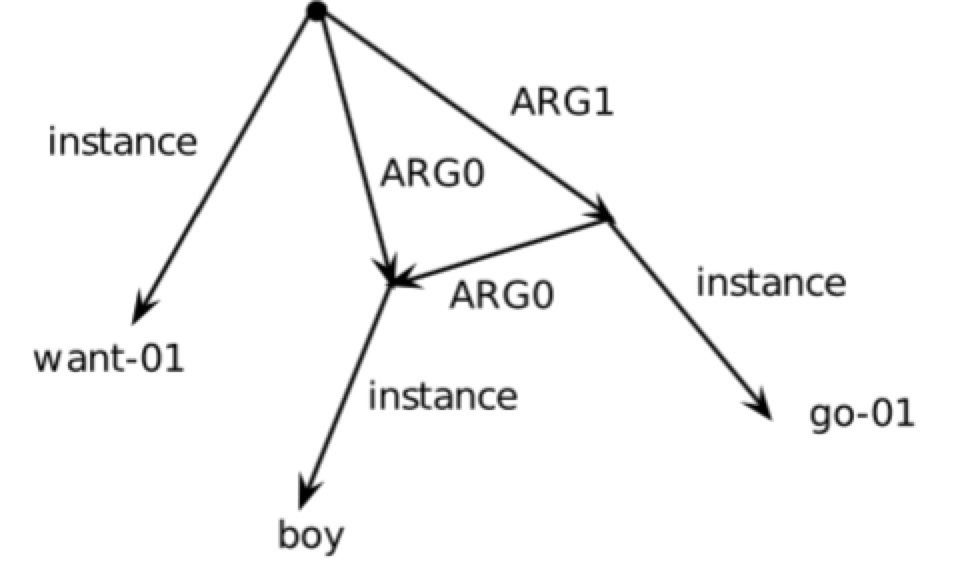
\includegraphics{graph_amr.png}
		\caption{图方式}
		\label{graph_format}
	\end{minipage}
   	\begin{minipage}
		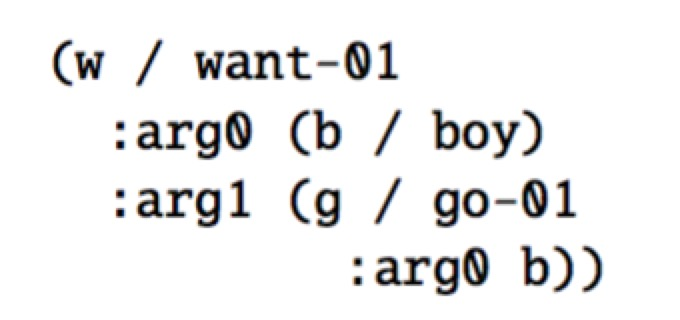
\includegraphics{text_amr.png}
		\caption{AMR文本方式}
		\label{graph_format}
	\end{minipage}
	\begin{minipage}
		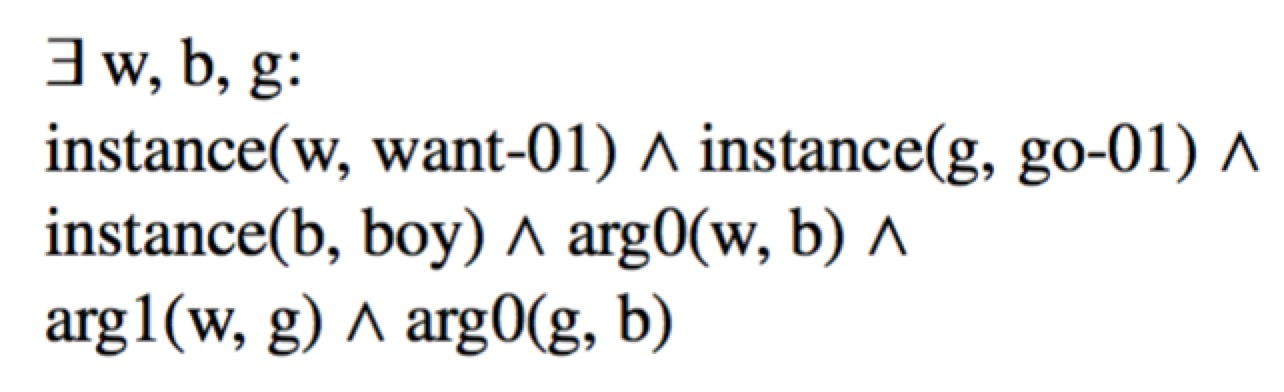
\includegraphics{logic_amr.png}
		\caption{逻辑三元组方式}
		\label{graph_format}
	\end{minipage}
\end{figure}

\subsection{翻译模型}\label{section:tmextract}
翻译模型,又叫短语表。短语表中存储的是双语短语对以及各个短语对之间的翻译概率\cite{marcu2002phrase}。在统计机器翻译中,短语指源语言句子或目标语言句子中连续的词序列,该词序列并不一定是语法意义上的短语。短语表是一个集合,该集合中每一个元素包括:源语言、目标语言短语对$(s,t)$、 短语对之间的短语翻译概率、词汇化翻译概率。

Koehn等人\cite{koehn2003statistical,koehn2009statistical}提出了抽取短语翻译系统中短语表的方法。该方法由于简单易用,实验效果佳等优势逐渐成为主流方法。使用该方法抽取短语表时,要求短语对与词对齐一致(Consistent with Word Alignment)。与词对齐一致的含义是:如果源端短语$s$ 中的所有词与目标端短语$t$都有对齐,并且在逆方向也满足此规则,那么称($s, t$) 与词对齐一致,可用公式\ref{equation:consistent} 表示。
\begin{equation}
  \label{equation:consistent}
  \begin{aligned}
    &\forall t_i \in t: (t_i, s_j) \in Align \Rightarrow s_j \in s \\
   &AND~\forall s_j \in s: (t_i, s_j) \in Align \Rightarrow t_i \in t \\
   &AND~\exists t_i\in t, s_j \in s: (t_i, s_j) \in Align
  \end{aligned}
\end{equation}
在抽取短语表时,需要抽取出所有满足以下原则的短语对:
\begin{enumerate}
  \item 抽取的短语对满足短语的定义,即应是连续的词序列。
  \item 抽取的短语对中不能出现没有词对齐的现象。
  \item 短语对内部的任意词对齐都不能超过任意一端短语。
\end{enumerate}

结合图\ref{figure:wordalign}对上述原则作解释:短语对("大公司", "big company"),("去了 一家", "in a")构成合法的短语对,因为源端短语和目标端短语都是原始句子中的连续词序列,包含两条词对齐,且短语对内部的词对齐都不超过任意一端短语;而(" 上班", "got a") 不构成合法的短语对,因为与源端词"上班"对齐的目标端词除了"got a" 之外还包括"job",超过了目标端短语,不满足第三个原则。

在抽取短语对的同时,更重要的是估计短语对之间的概率表。翻译概率表中主要包括短语翻译概率、词汇化翻译概率、词汇化调序概率等。

短语翻译概率,包括正向(源端到目标端)短语翻译概率、逆向(目标端到源端)短语翻译概率。常用的翻译概率的估计方法是极大似然估计。在计算短语对($s,t$)的正向短语翻译概率时,首先计算出该短语对是从多少个句对中抽取的,记为$count(s,t)$。 然后统计所有合法的短语对总数,$count$;最后使用$count$对$count(s, t)$作归一化操作,得到正向短语翻译概率(见公式\ref{equation:tprob})。类似地,逆向短语翻译概率$p(s|t)$的计算也使用极大似然估计,只是计算方向是从目标端到源端。

\begin{equation}\label{equation:tprob}
  p(t|s)=\frac{count(s,t)}{\sum_{t_i}count(s, t_i)}
\end{equation}

词汇化翻译概率,包括正向、逆向词汇化翻译概率。词汇化翻译概率描述的是短语内部词语之间相互翻译的概率,也属于一种基本的平滑方法。作为翻译模型中的一部分,词汇化翻译概率对机器翻译系统的性能同样有着重要影响。给定短语对($s,t$),在估计正向词汇化翻译概率时,同样需要基于词对齐进行极大似然估计,具体计算方法如公式\ref{equation:lexical}所示。

\begin{equation}
  \label{equation:lexical}
  p(t|s,a)=\prod_{i=1}^{length(t)} \frac{1}{|{j|(i,j) \in a}|} \sum_{\forall (i,j) \in a} w(t_i|s_j)
\end{equation}

其中,s, t分别为源端、目标端短语,a为词对齐,$(i,j) \in a$表示词对齐$a$包含$(t_i, s_j)$的对齐关系。$w(t_i|s_j)$表示词汇化翻译概率,其计算方法如公式\ref{equation:lexicalweight} 所示。类似地,逆向短语翻译概率$p(s|t,a)$的计算也使用极大似然估计,只是计算方向是从目标端到源端。

\begin{equation}
  \label{equation:lexicalweight}
  w(t_i|s_j)=\frac{count(t_i,s_j)}{count(s_j)}
\end{equation}
\subsection{词汇化调序模型}
词汇化调序模型\cite{tillmann2004unigram}考虑的是当前被翻译的源端短语A与前一个被翻译的源端短语B之间的相对位置关系。因为在短语机器翻译中,翻译是从左到右生成目标端的过程,每次选择一个源端短语进行翻译,并拼接到当前翻译之后,所以考虑当前源端短语A与前一源端短语B之间的相对关系相当于在翻译时考虑了挑选短语的顺序。我们通常考虑三种调序方向:单调调序(monotone, m),交换调序(swap, s),非连续调序(discontinuous, d),即$ p(orientation|s, t)$,其中$orientation \in \{m, s, d\}$。 具体地:
\begin{enumerate}
  \item 单调调序指A紧接着B之后。
  \item 交换调序指B紧接着A之后。
  \item 非连续调序指A与B不连续。
\end{enumerate}

在上述调序模型概念的基础上,对每个短语对的每一种调序类型,同样根据极大似然原理,统计每种情况出现的频率对调序模型进行参数估计。具体计算方法如公式\ref{equation:lrm}所示。

\begin{equation}
  \label{equation:lrm}
    p(orientation|s,t)=\frac{count(orientation,t,s)}{\sum_{orientation'} count(orientation',t,s)}
\end{equation}

最终,在实际使用中,由于短语翻译概率、词汇化翻译概率、词汇化调序概率都以短语对为基本单位,所以我们将三者统一整合到短语表中。

\subsection{语言模型}
语言模型刻画的是目标端语言句子可能出现的概率,它能够帮助机器翻译系统生成更流畅的译文。由于句子是连续的词序列,所以句子的概率可以用词的条件概率的连乘来刻画(如公式\ref{equation:lm})。当前主流的语言模型采用n 元文法($n$-gram)模型\cite{manning1999foundations}。根据马尔科夫有限视野假设,$n$ 元文法模型认为当前词的概率只与当前词之前的$n-1$ 个词相关,即$p(w_m|w_1,w_2...w_{m-1})=p(w_m|w_{m-n+1}...w_{m-1})$,所以在$n$ 元文法语言模型的限定下,给定一个长度为$m$ 的词序列,句子的概率可以近似地表示为公式\ref{equation:lmSimple}。 其中,$n$-gram 概率依然使用极大似然估计进行计算(公式\ref{equation:ngram} 所示),其中$count(w_1,...,w_m)$ 表示该词序列在单语语料中出现的次数。
\begin{equation}
  \label{equation:lm}
      p(w_1,...,w_m) = p(w_1)p(w_2|w_1)p(w_3|w_1,w_2)...p(w_m|w_1,...,w_{m-1})
\end{equation}
\begin{equation}
  \label{equation:lmSimple}
  p(w_1,...,w_m) \approx p(w_1|NULL)p(w_2|NULL,w_1)...p(w_m|w_{m-n+1},...,w_{m-1})
\end{equation}
\begin{equation}
  \label{equation:ngram}
  p(w_n|w_1,...,w_{n-1})=\frac{count(w_1,...,w_n)}{count(w_1,...,w_{n-1})}
\end{equation}

\section{参数训练}\label{section:parameter}
在第\ref{section:modeling}节中,我们介绍了机器翻译中的对数线性模型建模方法。在对数线性模型中,每一维特征$h$都应有一个对应的权重$w$,而$w$ 通常需要通过参数训练的方法来获取。

Och等人\cite{och2003minimum}于2003年提出最小错误率训练(Minimum Error Rate Training, MERT),用于训练机器翻译中对数线性模型的参数。
MERT需要使用一个小规模的双语平行语料(开发集,Development Set),该语料通常包括数百个互为翻译的句对。初始时,在参数空间中随机选择一组参数,翻译系统使用该组参数对开发集中所有句子进行解码并计算损失函数。接下来,选择某一维参数,固定其他参数,并以最小化损失函数为目标优化选中的参数。不断迭代以上过程直到满足终止条件(损失函数变化小于某阈值或迭代轮数超过某个阈值),从而获得最终参数。公式\ref{equation:mertloss} 给出了损失函数的形式。

\begin{equation}
  \label{equation:mertloss}
  L(T,R)=\sum_{i=1}^NL(t_i, r_i)
\end{equation}

其中$T$为整个开发集的翻译结果集合,$R$为整个数据集的参考译文集合,$N$为开发集句对数,$t_i$,$r_i$分别为第$i$ 个源语言句子的机器翻译输出结果和对应的参考译文。

公式\ref{equation:lossfunction}给出了最小化损失函数以求解最优参数的形式化表示:
\begin{equation}
  \label{equation:lossfunction}
  \begin{aligned}
    \lambda_1^M=\arg\min[\sum_{i=1}^NL(f(t_i,\lambda_1^M), r_i)]\\
    t'=f(s_i,\lambda_1^M)=\arg\max_{t\in c_i}[\sum_{m=1}^M\lambda_mh_m(s_i,t)]
  \end{aligned}
\end{equation}

其中$h_i$和$\lambda_i$分别表示第$i$维特征的特征值和其对应的权重;$t'=f(s_i,\lambda_1^M)$ 表示在给定模型参数$\lambda_1^M$ 的情况下,机器翻译系统解码开发集中第$i$ 个源语言句子$s_i$ 得到的最佳翻译译文(模型得分最高的译文);$c_i$ 表示$s_i$ 对应的所有可能的翻译译文。

\section{解码}
\label{section:decodeMethod}
解码(Decoding)即翻译。在短语机器翻译系统中,解码是使用翻译模型、语言模型、词汇化调序模型等搜索最佳译文的过程。与自然语言处理中很多问题类似,机器翻译的解码是一个结构化搜索问题,其搜索空间是指数级的,所以不可能穷尽整个搜索空间。我们需要一种复杂度更低的算法来搜索最佳译文。

Koehn等人\cite{koehn2009statistical}提出柱搜索算法(Beam Search)来降低搜索复杂度。柱搜索是一种启发式搜索算法,避免了全空间搜索,所以能够降低搜索复杂度。由于柱搜索不进行全空间搜索,所以会导致搜索到的最终解不是最优解,而是一个近似最优的解。

\subsection{解码流程}\label{section:decode}
我们首先以图\ref{figure:process}中的例子来解释短语系统的解码过程。第一行表示已经分词的源语言句子:“他~去了~ 一家~ 大公司~ 上班”。第二行中的每个方框里是一个源端短语,对应的下标表示该短语在解码时被选中的次序。第三行表示最终生成的翻译结果,每个方框中是一个目标端短语。系统首先选择源端短语“他”进行翻译,其对应的翻译结果为实线箭头所指向的英文部分("he");在翻译完“他”之后,系统可以按照源语言的顺序翻译“去了”,也可以不按照源语言的顺序而跳过若干词,先翻译后面的短语。在该例中,系统不按照源语言的顺序翻译,跳过若干词选择了“上班”,并将其翻译成"got a job",进而将这个翻译连接到之前的部分翻译之后,得到"he got a job"。系统不断选择未翻译的短语进行翻译,直至将最后一个未翻译的短语“大公司”翻译为"big company"并连接在部分翻译之后,从而生成最终的翻译结果"he got a job in a big company"。

\tikzstyle{block} = [rectangle, draw, text centered, minimum height=1.6em]
\tikzstyle{word} = [rectangle, text centered, minimum height=1.6em]
\tikzstyle{line} = [draw, -latex']
\tikzstyle{cloud} = [draw, ellipse, node distance=3cm, minimum height=2em]
\begin {figure}[ht]
\centering
\begin{tikzpicture}[auto, swap]
    % Place nodes
    \node [word] (w1) {他};
    \node [word, right of=w1, node distance =2cm] (w2) {去了};
    \node [word, right of=w2, node distance=2cm] (w3) {一家};
    \node [word, right of=w3, node distance=2cm] (w4) {大~~公司};
    \node [word, right of=w4, node distance=2cm] (w5) {上班};
    \node [block, below of=w1] (s1) {他$_1$};
    \node [block, below of=s1, node distance=2cm] (t1) {he};
    \node [block, below of=w5] (s2) {上班$_2$};
    \node [block, right of=t1, node distance=2cm] (t2) {got a job};
    \node [block, below of=w2] (s3) {去了$_3$};
    \node [block, right of=t2, node distance=2cm] (t3) {in};
    \node [block, below of=w3] (s4) {一家$_4$};
    \node [block, right of=t3, node distance=1cm] (t4) {a};
    \node [block, below of=w4] (s5) {大~~公司$_5$};
    \node [block, right of=t4, node distance=2cm] (t5) {big company};

     % Draw edges
    \footnotesize
    \path [line] (s1) -- (t1);
    \path [line] (s2) -- (t2);
    \path [line] (s3) -- (t3);
    \path [line] (s4) -- (t4);
    \path [line] (s5) -- (t5);
\end{tikzpicture}
\caption {\label{figure:process} 短语翻译过程示例}
\end{figure}

从例子中我们可以看到,短语翻译系统的解码是从左向右生成目标端的过程,生成的部分翻译一般被称为翻译假设(Hypothesis)。假设扩展指的是翻译系统选择未被翻译的源端短语,进而从翻译模型(或称为短语表)中挑选合适的翻译选项(Translation Option),并将其翻译连接到当前翻译假设之后,同时更新翻译假设模型得分的过程。由此可知短语翻译系统的解码过程实际上是不断进行假设扩展(Hypothesis Expanding)的过程。

给定一个输入源语言句子,翻译系统首先加载各种统计模型,进而迭代地从短语表中选取翻译选项进行假设扩展。当源语言句子中所有词都被翻译后,生成一个完整假设,完整假设中模型得分最高的被认为是最优翻译假设。

%\tikzstyle{decision} = [diamond, draw, aspect=1.5,
%    text width=5em, text badly centered, inner sep=0pt]
%\tikzstyle{block} = [rectangle, draw,
%    text width=5em, text centered, minimum height=1.6em]
%\tikzstyle{dashblock} = [rectangle, draw,dashed,
%    text width=8em, text centered, rounded corners, minimum height=1.6em]
%\tikzstyle{circle} = [rectangle, draw,
%text width=4em, text centered, rounded corners, minimum height=1.6em]
%\tikzstyle{line} = [draw, -latex']
%\tikzstyle{cloud} = [draw, ellipse, node distance=3cm,
%    minimum height=2em]
%\begin {figure}[ht]
%\centering
%\begin{tikzpicture}[node distance = 1.2cm, auto]
%    % Place nodes
%    \node [circle] (start) {源语言句子};
%    \node [block, below of=start, node distance=2cm] (option) {获取候选短语};
%    \node [block, left of=option, node distance=4cm] (lm) {语言模型};
%    \node [block, right of=option, node distance=4cm] (tm) {翻译模型};
%    \node [block, below of=option, node distance=2cm] (future) {未来代价估计};
%    \node [block, below of=future, node distance=2cm] (search) {柱搜索};
%    \node [decision, below of=search, node distance=2cm] (complete) {完整假设?};
%    \node [circle, below of=complete, node distance=2cm] (stop) {生成完整假设};
%    % Draw edges
%    \path [line] (start) -- (option);
%    \path [line] (lm) -- (option);
%    \path [line] (tm) -- (option);
%    \path [line] (option) -- (future);
%    \path [line] (future) -- (search);
%    \path [line] (search) -- (complete);
%    \path [line] (complete) -- node{是}(stop);
%    \path [line] (complete) -- node{否}(option);
%\end{tikzpicture}
%\caption {\label{figure:decoding} 解码流程图}
%\end{figure}

%---------------------------------------------------------------------------------------------------
\subsection{短语翻译中的柱搜索}
由于在假设扩展的过程中,可能有多个翻译选项可用于假设扩展,所以系统需要使用每一个可能的翻译选项进行假设扩展,这就导致了搜索空间的指数级增长。Koehn等人提出了基于栈的启发式搜索算法(柱搜索,Beam Search),通过在假设扩展的同时进行大量剪枝以达到降低解码复杂度的目标。

当翻译系统在进行假设扩展时,首先需要将选取的翻译选项的目标端连接到当前翻译假设的目标端之后,从而更新假设的目标端;其次,需要更新假设得分,并更新假设栈,同时根据假设得分进行栈剪枝。由于需要进行剪枝操作,而剪枝操作需要对剪枝的对象进行打分并将得分低的剪去,所以柱搜索算法就需要比较局部假设的得分。我们希望局部假设的比较相对公平,所以通常的做法是将翻译了相同数量的源端词的假设放在同一个栈中进行比较。在此基础上,为了进一步增强局部假设的可比较性,系统在计算局部假设的得分时,除了对数模型得分之外,通常还需要加上未来代价估计(Future Cost Estimation)得分。在进行栈剪枝时,不仅需要考虑假设得分,也要考虑假设重组的情况。我们将在下文中详细介绍上述内容。

\begin{algorithm}
\begin{algorithmic}[1]
\STATE Put empty hypothesis into stack 0
\FOR{all stacks from 0 to n-1}
    \FOR{all hypothesis in stack}
        \FOR{all translation options from phrase table}
            \IF{valid}
                \STATE Create new hypothesis;
                \STATE Recombine with existing hypothesis if possible;
                \STATE Place in corresponding stack;
                \STATE Prune stack if too big;
            \ENDIF
        \ENDFOR
    \ENDFOR
\ENDFOR
\end{algorithmic}
\caption{\label{algorithm:beamsearch}柱搜索伪代码}
\end{algorithm}

算法\ref{algorithm:beamsearch}给出了短语翻译系统中的柱搜索算法的伪代码。初始时将空假设放入0号栈,并开始假设扩展。对所有栈中的每一个假设,系统都从短语表中取出所有可用的翻译选项,并逐个用于假设扩展,从而生成新的假设,同时更新假设特征值、进行假设重组等。生成新的假设后,系统将新的假设加入到对应的栈中,然后根据假设得分进行栈剪枝等操作。由此可看出,柱搜索算法的复杂度为$O(n*b*m)$,其中$n$ 为句子长度,$b$ 为假设栈的大小,$m$ 为翻译选项数量。

\subsubsection{翻译选项}
翻译选项(Translation Options),或称为翻译候选,是指源端句子中的短语、该源端词短语在短语表中对应的目标端候选,这两者构成的短语对。短语表由第\ref{section:tmextract} 节中的方式按照词对齐信息事先抽取获得。对于源端句子$s$ 中的任意短语$s_i^j$\footnote{覆盖源端第$i$ 到第$j$ 个词的短语},只要在短语表中能够找到源端与$s_i^j$完全相同的翻译选项,就可以使用该翻译选项进行假设扩展。

由算法\ref{algorithm:beamsearch}可知,在翻译一个句子时需要遍历所有可能的翻译选项。为了降低复杂度,在抽取短语表时,通常的做法是对短语的最长长度进行限制。对于一个长度为$n$的源端词序列,我们通过将翻译选项的最长长度设置为固定值,就可以使合法翻译选项的规模降为$O(n)$。 进一步地,在假设扩展时引入扭曲限制(Distortion),限制短语候选的选取必须在当前假设的前后固定窗口大小$d$中,这就使得可用于假设扩展的合法翻译选项数降低到常数级。通常情况下,我们还会将假设栈的大小$b$设置为某个固定常数,所以柱搜索的复杂度为$O(n)$。

\subsubsection{假设剪枝与未来代价估计}
假设剪枝是指当假设栈的大小达到一定程度时,需要控制栈大小不再增长。通常的做法是把得分低的假设丢弃,得分高的假设加入栈中,这样就可以避免栈大小的无线增长,从而避免搜索空间的指数级增长,大大降低搜索复杂度。常用的方法包括直方图剪枝(Histogram Pruning)和阈值剪枝(Threshold Pruning)。

由于需要进行栈剪枝,虽然大大降低了搜索复杂度,但也带来了显著的搜索错误。系统可能将一些合理的假设剪掉,从而使得之后的假设无法使用这些合理的假设进行扩展。上文中我们描述到,同一个栈中存放的是翻译了相同数目源端词的假设,而非翻译了相同源端短语的假设,这就导致了局部假设的比较存在不公平性。因为不同的源端短语,即使它们的词数相同,它们的翻译难度或翻译代价是不同的。例如两个源端短语分别为“你好” 和 “第一次”,将“你好”翻译成"hi" 的对数线性模型得分比将“第一次”翻译成"the first time" 的得分高,但是这并不能证明前者的翻译更好。针对这样的问题,Koehn 等人又提出使用对数线性模型得分加上未来代价估计进行局部假设的得分估计的方法,目标是使局部假设的假设得分估计更准确。

\begin{algorithm}
\begin{algorithmic}[1]
\FOR{len from 1 ... n }
    \FOR{s from 1 ... n+1 - len}
        \STATE e = s + len
        \STATE cost(s, e) = INFINITE
        \IF{translation option (s, e) exists}
            \STATE cost(s, e) = score(s, e)
        \ENDIF
        \FOR{i from s ... e -1}
            \IF{cost(s, i) + cost(i + 1, e) < cost(s, e)}
                \STATE cost(s, e) = cost(s, i) + cost(i + 1, e)
            \ENDIF
        \ENDFOR
    \ENDFOR
\ENDFOR
\end{algorithmic}
\caption{\label{algorithm:futurecost}未来代价估计算法伪代码}
\end{algorithm}

未来代价估计是指预计系统选取了某个翻译选项用于假设扩展后,源端句子中还未翻译的部分的翻译代价或翻译难度。与对数线性模型得分类似,未来代价估计同样需要考虑翻译概率得分,语言模型得分和词汇化调序模型得分等。首先,翻译选项的翻译模型得分可以直接从短语表中获取;其次,由于系统无法得知未来翻译的真实情况,所以短语右边界的语言模型得分无法估计,从而只能考虑短语翻译内部的语言模型得分。最后,由于无法得知未来翻译的真实情况,所以无法得知短语翻译调序情况,所以在未来代价估计中忽略词汇化调序模型得分。我们将上述得分相加,在所有可能的估计值上选取代价最小的估计值作为未来代价估计。

未来代价估计的伪代码可以由算法\ref{algorithm:futurecost}表示。对于所有未被翻译的源端词区间,如果存在恰好可以覆盖当前区间的翻译选项,则使用该翻译选项的得分表示该区间的未来代价;否则,将该区间划分成若干个子区间,使用能够恰好覆盖其子区间的翻译选项的得分之和作为未来代价,最终选取所有可能的未来代价的最小值作为最终未来代价估计值。

\subsubsection{假设重组}
为了进一步降低搜索空间,提高假设之间的可比较性,短语翻译系统在假设扩展时通常还需要进行假设重组(Hypothesis Recombination)。当两个局部假设$H_1$ 和$H_2$ 翻译了相同的源端部分,但是两个假设由两个不同翻译路径产生时,可能会导致其中一个假设$H_1$的局部得分比另一个假设$H_2$ 的得分高。当满足一定条件时,在之后的假设扩展中,经过$H_1$ 扩展的假设$H_1'$永远比经过$H_2$扩展的假设$H_2'$高,此时由于再扩展$H_2$ 已经没有意义,所以将$H_1$ 和$H_2$ 进行假设重组,丢弃得分低的假设$H_2$,保留得分高的假设$H_1$。

在现有的短语机器翻译系统中,需要保证两个假设$H_1$,$H_2$的某些特征完全一致才能够保证当前得分更高的假设在后续扩展时得分仍然更高,具体地:
\begin{enumerate}
  \item $H_1$和$H_2$覆盖的源端相同,保证待翻译的内容一致。
  \item 在使用$n$元文法条件下,$H_1$和$H_2$的最后$n-1$个翻译词相同,保证后续扩展的语言模型得分一致。
  \item $H_1$和$H_2$最后翻译的源端短语相同,保证调序模型得分一致。
\end{enumerate}

\section{自动评价指标}
\label{section:measurement}
人工评价虽然评价效果优,但是由于效率低、昂贵等缺陷,无法使用在大规模机器翻译评测任务中。常用的机器学习问题评价指标,准确率、召回率难以被直接使用到机器翻译的译文自动评价中。因为在机器翻译系统译文评价中,单词之间的位置关系显然应该是重要的评价标准之一,但准确率和召回率都无法描述翻译单词之间的位置关系信息。合理的机器翻译评价标准不仅应该可以体现准确率、召回率,而且应该体现出翻译顺序的正确程度。

Papineni等人\cite{papineni2002bleu}于2002年提出Bilingual Evaluation Understudy, BLEU。BLEU 中不仅包含了单词的准确率、召回率等信息,还包括了词序信息。由于其简单易用,与人工评价的一致性高等优势,自2002年以来一直是机器翻译系统译文自动评价方法中使用最广的方法之一。

BLEU的计算方法中,首先需要计算的是$n$ 元文法的匹配准确率,公式\ref{equation:bleupre} 给出了$n$元BLEU的计算方法。
\begin{equation}
  \label{equation:bleupre}
  BLEU_n = exp[\sum_{i=1}^n\lambda_ilog(p(i))]
\end{equation}

其中,$\lambda_i$为$i$元文法的权重,一般情况下都取值为1,$p(i)$为$i$元文法的匹配率。由此可知BLEU 得分与$n$ 元文法的匹配程度成正比。我们通常基于整个数据集来计算BLEU 得分。

在公式\ref{equation:bleupre}的基础上,引入一个基于长度的惩罚项,该惩罚项表示:生成译文与参考译文的单词数越接近,则生成译文质量越高(如公式\ref{equation:bleu}所示)。其中,$r$, $c$分别代表参考译文的长度和翻译译文的长度。

\begin{equation}
  \label{equation:bleu}
    \begin{aligned}
  BLEU_n=BP*exp[\sum_{i=1}^n\lambda_ilog(p(i))]\\
  BP=\min(1,exp(1-\frac{r}{c}))
  \end{aligned}
\end{equation}

\section{本章小结}
本章主要介绍了基于短语的统计机器翻译系统的各部分重点内容。首先介绍了短语机器翻译的整体框架与流程。在此基础上,分别介绍了短语机器翻译的建模方法,参数训练方法,解码方法等内容。

短语翻译系统通过最小错误率训练进行对数线性模型的参数调节,在开发集上,直接对翻译评价指标进行参数调节,每次调节一维参数,经过多轮迭代获得最优参数。统计机器翻译最常用的自动评价指标为BLEU。

短语翻译系统采用了对数线性模型进行建模,可以自然地使用各种特征。短语翻译系统主要使用了翻译概率、词汇化调序概率、语言模型概率、词计数、短语计数等特征。为了减少搜索空间,降低搜索复杂度,短语翻译系统采用了一种启发式搜索算法:柱搜索解码算法。柱搜索算法通过源端词数维护搜索栈,即翻译了相同源端词数的假设置于同一个栈中。柱搜索算法的核心是假设扩展和假设剪枝。翻译系统通过将翻译选项的目标端连接到局部假设之后,并同时更新假设的各项特征值来进行假设扩展。翻译系统通过局部假设的特征值得分和未来代价估计相加进行局部假设的得分估计,并使用该得分估计进行剪枝,提高了局部假设之间的可比较性,从而降低了搜索错误。在假设扩展过程中,为了进一步减少搜索空间,翻译系统通过假设重组,丢弃无效假设。

本文中提出的交互式机器翻译相关内容均建立在短语翻译系统的基础上,特别是短语翻译系统的短语表、解码方法、模型参数训练等内容上。对短语机器翻译系统中的关键部分的理解有助于对本文的理解。

\chapter{交互翻译框架}
\label{chapter:primt}
\section{引言}
传统的交互式机器翻译采用自左向右(Left-to-right, L2R)的交互框架。在第\ref{section:imtnow}节中我们描述到,在L2R交互框架中,给定一个待翻译源语言句子,用户可以自左向右进行翻译补全或错误修正,系统根据用户确认的正确翻译前缀提供后续翻译的补全建议。

虽然自左向右的交互框架取得了成功,但是该框架存在一个潜在的弱点,即该框架难以直接修正句末的关键翻译错误。关键错误是指对句子中其他词或短语的翻译质量有巨大影响的翻译错误。关键错误经常是由翻译源端短语的内在困难性导致的。Mohit等人\cite{mohit2007localization}于2007年提出了使用分类器来识别难以翻译的短语(Difficult-to-translate Phrases, DTPs)的方法。这项工作证明了让真实用户翻译DTPs比让用户翻译其他短语能够带来更显著的翻译质量的提升。关键错误与DTPs有类似的性质。

当一个翻译歧义点出现在句末,并且这个翻译歧义点引起了句末的关键错误,而该关键错误又导致了句首的翻译错误时,从左到右进行翻译修正就会延迟对该关键错误的修正,从而可能导致交互效率的低下。首先修正这个关键错误可能会对之前的翻译带来很大的正面影响,这样就可以在交互翻译的过程中显著减少人工代价。

在上述背景下,本章提出了一种新的交互式机器翻译框架,在该框架下,用户可以使用两种简单的操作完成交互翻译:选择一个关键翻译错误,修正该翻译错误。我们称这种框架为选择- 修正(Pick-Revise, PR)交互翻译框架。用户操作不局限于自左向右的框架,可以在句子的任意位置选择短语并修正其翻译,以此来提高人机交互效率。
\section{选择-修正交互框架}
\subsection{选择-修正交互翻译系统}
首先,我们用表\ref{table:example}来解释PR框架与L2R框架\cite{foster2002user}之间的区别。在该例子中,我们分别使用PR 框架和L2R 框架进行一次交互。第一行表示已分词的中文句子和每个词对应的英文翻译,接下来每一行分别表示参考译文、基线系统的翻译结果、一次L2R交互的翻译结果、一次PR 交互的翻译结果。虚线下划线表示L2R 框架修正的错误;实线下划线表示PR框架修正的错误;加粗的部分表示修正了翻译错误并重新解码后,对其他部分的翻译带来的正面影响。

\begin{table*}[!htb]
\footnotesize
\begin{center}
\begin{tabular}{l|l}
\hline
    \multirow{2}*{源端} &~~~~~~~南亚~~~~~~~~~~各国~~~~~~~~~~~~~外长~~~~~~~~~~~~~~~\dashuline{商讨}~~~~自由~~~~
    贸易区~~~~~和~~~~~\underline{反~~~~~~~~恐}~~~~~~~~问题\\
                \cline{2-2} & (south asian)(countries)(foreign minister)(discuss) (free)(trade
                zone)(and)(anti)(terrorism)(issue)\\
\hline
    参考译文& south asian foreign ministers discuss free trade zone and anti-terrorism issues\\
\hline
    基线& south asian foreign ministers \dashuline{to discuss} the issue of free trade area and
    \underline{the}\\
\hline
\hline
    L2R & south asian foreign ministers \dashuline{discuss} the issue of free trade area and the\\
\hline
\hline
    PR & south asian foreign ministers \textbf{discuss free trade area and} \underline{anti-terrorism} issues \\
\hline
\end{tabular}
\end{center}
\caption{\label{table:example} 使用L2R框架和PR框架修正中英翻译的例子}
\end{table*}

对于给定的源语言句子,短语翻译系统首先生成了一个基线翻译。在L2R框架下,用户修正最左端的错误,将"to discuss" 修改为"discuss",但这个修正并没有对其他部分带来正面影响。句子的翻译质量仍然未满足用户需求,所以用户需要更多操作来提升翻译质量。在PR框架下,用户认为"反~恐"是最关键的翻译错误进而选择该短语,并根据短语表将其翻译从"the"修改为"anti-terrorism"。限制解码器(Constrained Decoder)接收到用户信息并重新翻译该句子,不仅将该短语翻译正确,而且还提升了该短语翻译附近的翻译质量(粗体部分),带来了翻译顺序的改善。与L2R框架相比,PR 框架能够直接对关键错误进行修正,提升了用户交互的效率。

\tikzstyle{decision} = [diamond, draw, aspect=1.5,
    text width=5em, text badly centered, inner sep=0pt]
\tikzstyle{block} = [rectangle, draw,
    text width=8em, text centered, rounded corners, minimum height=1.6em]
\tikzstyle{dashblock} = [rectangle, draw,dashed,
    text width=8em, text centered, rounded corners, minimum height=1.6em]
\tikzstyle{circle} = [rectangle, draw, text width=4em, text centered, rounded corners, minimum height=1.6em]
\tikzstyle{line} = [draw, -latex'] \tikzstyle{cloud} = [draw, ellipse, node distance=3cm,
    minimum height=2em]
\begin {figure}[!htb]
\centering
\begin{tikzpicture}[node distance = 1.8cm, auto]
    % Place nodes
    \small
    \node [circle] (start) {开始};
    \node [block, below of=start] (constrain) {限制解码器};
    \node [block, right of=constrain, node distance=4.2cm] (rev) {修正};
    \node [decision, below of=constrain, node distance=2cm] (decide) {可接受?};
    \node [block, right of=start, node distance=4.2cm] (learn) {模型自适应};
    \node [block, right of=decide, node distance=4.2cm] (pick) {选择};
    \node [circle, below of=decide, node distance=2cm] (stop) {结束};
    % Draw edges
    \small
    \path [line] (start) -- node{$s_1 ... s_n$}(constrain);
    \path [line] (constrain) -- node{$e_1 ... e_n$}(decide);
    \path [line] (decide) -- node [near start] {否} (pick);
    \path [line] (pick) -- node{($s_{i}^{j}$,$t$)}(rev);
    \path [line] (rev) -- node{($s_i^j$,$t'$)}(constrain);
    \path [line] (decide) -- node {是}(stop);
    %\draw [->,dashed] (rev) -- node{($s_i^j$,$t'$)}(learn);
    %\draw [->,dashed] (learn) -- (constrain);
    \path [line] (rev) -- node{($s_i^j$,$t'$)}(learn);
    \path [line] (learn) -- (constrain);
\end{tikzpicture}
\caption {\label{figure:framework} PRIMT框架流程图}
\end{figure}

图\ref{figure:framework}展示了我们的PR交互框架的整体流程图。给定一个源语言句子$s_1 ... s_n$和该句的初始翻译,用户首先从整句中选择一个翻译错误,然后选择一个短语表中存在的正确翻译结果。如果短语表中不存在正确的翻译,用户也可以自行输入翻译结果来替代错误的翻译结果。系统随后获取该信息,将该信息作为解码的限制,重新翻译该句。PR框架迭代地使用限制解码器生成新翻译,限制信息来自于先前的PR过程。PR 过程中产生的信息还将被用于进行模型自适应。整个交互过程一直持续到用户认为当前翻译结果已经可接受为止。我们将在下文中解释该框架中的关键内容。
\subsection{选择}
在选择(Picking)步骤中,用户选择翻译错误的短语($s_i^j$, $t$)(覆盖了源端第$i$个词到第$j$个词,并且翻译为$t$的短语对)进行修正。选择步骤的目标在于寻找翻译中由短语表的错误或内在的翻译歧义导致的关键错误。错误越关键,修正该错误带来的翻译质量的提升就越大\cite{mohit2007localization}。

为了使得选择步骤更容易被加入到机器翻译系统中,我们限制用户只能从上一次PR周期的输出中选择翻译错误。如果是第一次PR周期,那么用户只能从基线翻译系统的输出中选择翻译错误。为了让用户可以更便捷地进行交互,在我们当前的系统中,用户既可以从源端进行选择,也可以从目标端进行选择,用户只需进行简单的鼠标点击操作即可完成交互。我们的系统将源端与目标端的对应或对齐关系进行了可视化,使得用户更容易观察。

Green等人\cite{green2014human}的实验结果证明,让真实用户进行后编辑操作可以比进行L2R交互翻译更快地得到可接受的翻译结果。这样的结果也表明了识别关键错误对于真实用户而言并不困难。
\subsection{修正}
在修正(Revising)步骤中,用户从短语表中选取正确的翻译选项,将$s_i^j$的翻译修正为$t'$。当短语表中没有正确翻译选项时,用户也可以手动输入正确翻译。用户是否需要自己添加一个正确翻译选项由短语表的质量决定。当翻译系统由足够大的平行语料训练得到时,短语表的质量通常能够达到提供正确翻译的需求。

对于一个选择了的短语,短语表的翻译选项可以以列表的形式呈现给用户。用户只需要使用鼠标点击正确的翻译结果即可,用户也可以在输入框中另行输入一个短语翻译。
\subsection{解码器和模型自适应}
对于一个源端句子,在一个PR周期后,一个“选择-修正对” (Pick-Revise Pair, PRP)就可以被系统捕获。我们使用了一个限制解码器来根据之前捕获的PRP作为限制来搜索到新的最佳译文。PR框架中的限制解码算法与典型的短语翻译系统中的柱搜索解码算法类似,但是多了一个比较操作,该比较操作使解码算法忽略与PRP有冲突的翻译选项。

判断一个翻译选项是否与PRP有冲突的方法如下:
\begin{enumerate}
  \item 若一个翻译选项的源端与某个PRP的源端完全一致,且该翻译选项的目标端与PRP的目标端不一致,则该翻译选项与PRP有冲突。
  \item 若一个翻译选项的源端与某个PRP的源端有重叠,但不完全一致,则该翻译选项与PRP有冲突。
  \item 其他情况均无冲突。
\end{enumerate}

由于在限制解码算法中,所有与PRP有冲突的翻译选项都被系统忽略,所以整个搜索空间就比标准解码过程小了很多。在这样的设置下,我们就可以确保用户提供的PRP都能够被完全正确地翻译出来,并且确保整个过程可以实时进行。限制解码算法的伪代码由算法\ref{algorithm:prconstrain}给出,其中CONFLICT 函数即为判断当前翻译选项与PRP 是否冲突的函数。我们可以给出CONFLICT函数的伪代码(算法\ref{algorithm:conflict1})。

\begin{algorithm}
\begin{algorithmic}[1]
\REQUIRE ~~ \\
源端句子: $s_1 ... s_n$\\
PRP: ($s_i^j, t'$)\\
用于假设扩展的翻译选项: ($s_a^b, t$)
\ENSURE ~~ \\
新翻译$t_1' ... t_m'$
\WHILE{$Hypothesis~Expanding$}
\IF{$CONFLICT((s_a^b, t) , (s_i^j, t'))$}
    \STATE continue;
\ENDIF
\STATE Expand Hypothesis Using ($s_i^j, t'$);
\ENDWHILE
\end{algorithmic}
\caption{PR框架中的限制解码算法}
\label{algorithm:prconstrain}
\end{algorithm}

\begin{algorithm}
\begin{algorithmic}[1]
\REQUIRE ~~ \\
PRP: ($s_a^b, t$)\\
当前用于假设扩展的翻译选项: ($s_i^j, t'$)\\
\ENSURE~~\\
翻译选项与PRP是否有冲突
\STATE $CONFLICT((s_a^b, t) , (s_i^j, t'))$
\IF{$j >= a$ and $b >= i$}
    \IF {$a == i$ and $b == j$ and $t == t'$}
        \RETURN FALSE;
    \ENDIF
    \RETURN TRUE;
\ENDIF
\RETURN FALSE;
\end{algorithmic}
\caption{选择-修正中的冲突判断}
\label{algorithm:conflict1}
\end{algorithm}

系统可以捕获到所有PRP,在捕获到一定数量的PRP后进行模型自适应,重新训练模型,从而提升翻译系统本身的性能。我们将在后续章节中详细介绍本文提出的模型自适应方法。

\section{实验及结果分析}
\label{experiment:primt}
\subsection{实验配置}
在所有实验中,我们使用了一个自主研发的短语翻译系统来进行中英翻译。我们将选择-修正交互翻译框架加入到短语翻译系统中。用于训练翻译模型的双语平行语料包括820 万句对(LDC2002E18, LDC2003E14, LDC2004E12, LDC2004T08, LDC2005T10, LDC2007T09)。我们训练了一个$5$元文法的语言模型,并使用Modified Kneser–Ney平滑\cite{chen1999empirical},其训练数据为Gigaword的Xinhua部分,包含了1,460万英文句子。我们使用NIST02 和NIST03 两个开发集的并集来训练翻译系统的参数。我们使用NIST04和NIST05作为测试数据。翻译质量的自动评估使用不区分大小写的$4$ 元文法BLEU。 我们的系统的表现与领先的开源短语翻译系统Moses\cite{koehn2003statistical} 具有可比性。

\subsection{实验方法}
\label{sec:simulate}
因为真实的人工交互代价昂贵且耗费时间,所以我们在实验中使用模拟人工交互进行选择和修正操作。

在没有人工标注的情况下,在翻译中直接识别关键错误是一个困难的任务。我们将直接识别关键错误的任务转化为判断给定错误在其上下文下对翻译的影响的任务,以此来寻找关键错误。
具体地,对于一个句子,我们依次选择基线系统输出的每一个短语,然后使用模拟修正方法(将在下文描述)修正其翻译,系统进行限制解码后,我们就可以获得新翻译。新翻译的质量与原始翻译的质量的差异就可以衡量该短语对翻译质量的影响程度。我们将提升翻译质量最明显的短语作为模拟人工选择的结果。由于BLEU是最常用的机器翻译评价方法,所以我们选取使得BLEU提升最多的短语作为模拟人工选择的结果。

在没有人工标注的情况下,给定一个源语言短语,模拟修正操作相对模拟选择操作更为直接。具体地,在所有正确的翻译选项中(关于正确的翻译选项的定义见第\ref{sec:rsmtraining} 节),我们选择最长的翻译选项作为模拟人工修正的结果。

在选择-修正交互操作下,一个PR周期只需用户点击两次鼠标,不需要键盘输入。为了比较公平,我们对L2R框架使用相同的模拟修正操作,只是在使用L2R 框架时,从左向右地选择翻译错误并修正其翻译,所以每个L2R 周期也需要用户点击两次鼠标。同样地,我们选择最关键的错误作为后编辑(Post-Edit, PE)修正的对象。由于PE的过程只是字符串的修改,所以PE 系统每次交互所需要的键盘输入次数是正确短语翻译的字符数。

\subsection{理想环境下翻译质量提升}
第一组实验用于测试选择-修正交互翻译框架在理想环境下的性能表现。我们在使用当前系统进行强制解码可以成功解码出参考译文的句子上开展实验。强制解码是指强制翻译系统生成与参考译文完全一致的翻译结果。一个句子的参考译文可以通过强制解码产生,意味着这个句子不需要输入新单词来生成正确的翻译,这与我们的模拟实验中不要求用户输入正确翻译结果,只在短语表中选择翻译候选的设计方法一致。

NIST04和NIST05中分别有186 句和92 句可以成功强制解码。表\ref{table:forced}中PR*$n$表示系统进行$n$轮PR交互操作;PE系统对最关键的错误进行后编辑操作;L2R 系统修改最左端的错误。实验结果表明,选择并修正最关键的错误(PR*1)可以在NIST04 (forced)和NIST05 (forced)两个数据集上分别带来+18 和+13 BLEU 的提升,此时KSMR都是2.2\%。 选择最左错误 (L2R*1)并修正其翻译结果,同样需要2.2\%KSMR,但在两个数据集上都只带来+5 左右的BLEU 提升。这样的结果证明了选择关键错误在PR 框架下非常关键。对比L2R 方法,我们的PR 框架有可以优先处理关键错误的优势,优先修正这些错误,BLEU 的提升相比自左向右的修正更大。

\begin{table}[!htb]
\begin{center}
\begin{tabular}{c|c|c|c|c}
\hline
\multirow{2}*{数据} & \multicolumn{2}{c|}{NIST04 (forced)} & \multicolumn{2}{c}{NIST05 (forced)}\\
\cline{2-5} & BLEU& KSMR & BLEU & KSMR \\
\hline 基线 & 44.59& 0 & 41.48 & 0 \\
\hline PR*1 & \textbf{63.21 (+18.62)} &2.2 & \textbf{55.10 (+13.62)} & 2.2 \\
\hline PR*2 & \textbf{70.82 (+26.23)} &4.3 &\textbf{63.03 (+21.55)} & 4.4 \\
\hline PR*3 & \textbf{73.99 (+29.50)} &6.5 &\textbf{68.56 (+27.08)} & 6.7 \\
\hline PR*4 & \textbf{75.48 (+30.89)} &8.6 & \textbf{72.20 (+30.72)} & 8.9 \\
\hline PR*5 & \textbf{76.59 (+32.00)} &10.8 & \textbf{73.90 (+32.42)} & 11.1 \\
\hline PR*6 & \textbf{78.07 (+33.48)} &12.9 & \textbf{75.22 (+33.74)} & 13.3 \\
\hline PR*7 & \textbf{79.27 (+34.68)} &15.1 & \textbf{75.57 (+34.09)} & 15.5 \\
\hline PR*8 & \textbf{79.54 (+34.93)} &17.2 & \textbf{76.02 (+34.54)} & 17.8 \\
\hline
\hline L2R*1 & 49.32 (+4.73) & 2.2 & 46.34 (+4.86) & 2.2 \\
\hline PE*1 & 49.77 (+5.18) & 8.3 & 46.81 (+5.33) & 8.2 \\
\hline
\end{tabular}
\end{center}
\caption{\label{table:forced} 理想环境下的交互翻译结果}
\end{table}
\label{sec:translationquality}

后编辑最关键错误(PE*1)需要8\% KSMR,但只带来+5 BLEU左右的提升。对比于无法影响周边翻译的后编辑方法,我们的PR 框架可以重新解码获得更好翻译,从而减少用户交互。

持续进行PR交互能够持续提升翻译质量。在8次PR周期后(PR*8,约17\% KSMR),我们的系统对比基线系统,在两个数据集上都带来了约+35 BLEU的提升,达到了75 BLEU左右,这样的翻译结果质量已经非常高。这样的结果证明了用户在使用选择- 修正交互翻译系统进行交互翻译时,使用较少的交互次数即可获得高质量的翻译结果。

\subsection{通用环境下翻译质量提升}
我们也在通用环境下(NIST04和NIST05整个数据集)验证选择-修正交互翻译框架的性能表现。

\begin{table}[!htb]
\begin{center}
\begin{tabular}{c|c|c|c|c}
\hline
\multirow{2}*{数据} & \multicolumn{2}{c|}{NIST04} & \multicolumn{2}{c}{NIST05}\\
\cline{2-5} & BLEU& KSMR & BLEU & KSMR \\
\hline 基线 & 31.83 & 0 & 30.64 & 0 \\
\hline PR*1 & \textbf{42.88 (+11.05)} &1.1 & \textbf{41.47 (+10.83)} & 1.1 \\
\hline PR*2 & \textbf{48.21 (+16.38)} &2.2 & \textbf{45.76 (+15.12)} & 2.2 \\
\hline PR*3 & \textbf{50.12 (+18.29)} &3.3 & \textbf{48.33 (+17.69)} & 3.3 \\
\hline
\hline L2R*1 & 35.61 (+3.78) & 1.1 & 33.85 (+3.21) & 1.1 \\
\hline PE*1 & 34.74 (+2.91) & 4.3 & 34.18 (+2.54) & 4.8 \\
\hline
\end{tabular}
\end{center}
\caption{\label{table:frameAbility} 通用环境下的交互翻译结果}
\end{table}

表\ref{table:frameAbility}给出了实验结果,表中各行的意义与表\ref{table:forced}一致,唯一的区别在于第一行的NIST04和NIST05表示这两个数据集的全部句子,而不仅仅是其中可以成功强制解码的句子。

通用环境下,NIST04和NIST05两个数据集的BLEU提升比理想环境低,导致这种现象的原因主要有两点:一是在通用环境下,句子的复杂性通常较高,短语翻译系统本身的能力限制了PR交互框架对BLEU的提升能力;二是在通用环境下,由于当前翻译系统的统计模型并不完美,所以当前的短语表可能无法涵盖所有短语的正确翻译,从而可能需要用户输入正确翻译结果。而我们的模拟交互方法并没有使用真实用户进行翻译,只模拟让用户从短语表中选择翻译选项的情况,并不模拟让输入正确的翻译结果的情况。让真实用户输入短语表中不存在的正确翻译结果可以进一步提升翻译质量。

尽管通用环境下BLEU提升比理想环境低,但是实验结果仍然展示了与理想环境中类似的趋势。一次PR周期(PR*1)可以在NIST04和NIST05两个数据集上都带来+11 左右的BLEU提升。持续进行PR交互可以持续提升翻译质量。三次 PR 周期只需约3.3\% KSMR,却可以获得+17 的BLEU 提升。一次L2R交互(L2R*1)和一次PE操作(PE*1)分别在两个数据集上只带来+3.2和+2.5左右的BLEU提升。这样的结果证明,对比L2R 和PE 框架,我们的框架在通用环境下仍然有显著优势。

%\subsection{使用自动建议模型}
%我们在本组实验中通过分类器表现和翻译表现两方面验证自动建议模型的有效性。
%
%表\ref{table:ASMC}中展示了使用不同分类器建模两种自动建议模型时的表现,每个单元格中的三个数值分别代表准确率、召回率和F度量。准确率和召回率都基于测试集中的正例计算而得,因为只有被预测为正例的实例才可以被用于交互机器翻译系统中。因为自动确定正确的翻译选项是一个较难的任务,所以当所有翻译选项都被预测为负例时,我们保持原先翻译选项不变。
%
%\begin{table}[!htb]
%\begin{center}
%\begin{tabular}{c|c|c|c}
%\hline 建议模型 & 分类器 & NIST04 & NIST05\\
%\hline
%\multirow{3}*{选择建议模型} & 最大熵 & 0.70/0.62/0.66 & 0.69/0.60/0.64\\
%            \cline{2-4}& 支持向量机 & 0.71/0.68/0.69 & 0.69/0.66/0.67\\
%            \cline{2-4}& 前馈神经网络 & 0.71/0.73/0.72 & 0.68/0.70/0.69\\
%\hline
%\hline
%\multirow{3}*{修正建议模型} & 最大熵 & 0.71/0.58/0.63 & 0.70/0.57/0.63\\
%            \cline{2-4} & 支持向量机 & 0.70/0.61/0.0.65 & 0.68/0.62/0.65 \\
%            \cline{2-4} & 前馈神经网络 & 0.66/0.67/0.66  &0.65/0.65/0.65 \\
%\hline
%\end{tabular}
%\end{center}
%\caption{\label{table:ASMC} 自动建议模型的分类器表现}
%\end{table}
%
%由表中数据可知,三种分类器的表现相近,前馈神经网络稍有优势。选择建议模型可以以F-度量值0.67来识别关键错误;修正建议模型可以以F-度量值0.65 来识别正确翻译。因为两个任务的难度都较大,所以F度量都在0.60和0.70之间是可接受的。
%
%我们也测试了在PR框架下使用自动建议模型进行交互翻译的表现(见表~\ref{table:ASMT})。如果随机选择一个源端短语进行模拟修正,BLEU几乎无提升。相比而言,使用选择建议模型并进行模拟修正可以在两个数据集上都获得显著提升(+2 BLEU左右)。这表明了BLEU提升并不来源于模拟修正的参考译文匹配长度,选择操作在PR 框架下非常关键。选择最关键的错误后,随机修正也无法带来BLEU提升,而使用修正建议模型可以提升1.5 BLEU。
%
%\begin{table}[!htb]
%\begin{center}
%\begin{tabular}{c|c|c|c}
%\hline &  & NIST04 & NIST05\\
%\hline & 基线 & 31.83 & 30.64\\
%\hline
%\hline & 随机选择 &  31.92 (+0.09) & 30.69 (+0.05)\\
%\hline \multirow{3}*{选择建议模型} & 最大熵 & 33.89 (+2.06) & 32.57 (+1.93)\\
%                    \cline{2-4}  & 支持向量机 & 34.01 (+2.18) & 32.66 (+2.02) \\
%                    \cline{2-4}  & 前馈神经网络 & 34.23 (+2.40) & 32.81 (+2.17) \\
%\hline
%\hline & 随机修正 & 31.90 (+0.07) & 30.71 (+0.08)\\
%\hline
%    \multirow{3}*{修正建议模型} & 最大熵 & 33.62 (+1.79) & 32.38 (+1.74)\\
%                    \cline{2-4}  & 支持向量机 & 33.73 (+1.90) & 32.42 (+1.78)\\
%                    \cline{2-4}  & 支持向量机 & 33.77 (+1.94) & 32.44 (+1.80) \\
%\hline
%\end{tabular}
%\end{center}
%\caption{\label{table:ASMT} 随机选择和使用自动建议模型下的翻译质量变化情况}
%\end{table}
%
%使用任意一种建议模型都可以提升翻译质量,此时用户只需要进行一种操作(选择或修正)。这种情况下可能更适用于单个用户操作。诚然,使用某一种自动建议模型时,翻译质量的提升较全部使用模拟交互更小,这表明了用户的参与仍然对于翻译质量的提升至关重要。我们可以使用更好的模型、更大的数据量来提升自动建议模型的质量。

\section{本章小结}
本章提出了一种选择-修正的交互式机器翻译框架(Pick-Revise IMT, PRIMT),在该交互翻译框架下,用户只需要进行两种简单的交互操作即可完成交互翻译。用户可以选择句子中任意位置的关键错误并修正其翻译,以此提高交互翻译效率。

实验结果证明优先修正关键错误而非最左翻译错误,可以使我们的框架可以更快、更有效率地提升翻译质量。用户使用选择-修正交互翻译框架进行交互翻译,使用较少的交互操作就能获得高质量的翻译结果。进一步提升选择- 修正框架的方法有多种,主要包括:支持其他类型的交互,使用更强的统计模型等方法。
%实验结果证明修正关键错误而非最左翻译错误,使我们的框架可以更快、更有效率地提升翻译质量。在此基础上,我们针对用户的两种操作提出两个自动建议模型。使用自动建议模型可以将用户的操作进一步简化为一种操作(选择或修正)。让不同的用户负责不同的操作,可以使用户专注于某一种操作,这更适合真实用户使用。进一步提升选择-修正框架的方法有多种,主要包括:支持其他类型的交互,使用更强的统计模型等。
\chapter{自动建议模型}
\label{chapter:asm}
\section{引言}
在第\ref{chapter:primt}章中,我们描述了基于短语翻译系统的选择-修正(PR)交互翻译框架。与传统的L2R交互翻译框架不同,在该框架下,用户可以使用两种简单的操作(选择与修正)即可直接修正任意位置的关键错误,以此提升翻译质量和交互效率。

Ueffing 等人于2003 年提出统计机器翻译中的置信度度量(Confidence Measure)\cite{ueffing2003confidence}。给定一个源语言句子及对应的机器翻译系统生成的翻译结果,置信度度量要预测的是翻译结果中每个翻译单元是正确翻译的概率。在置信度度量中,翻译单元是每个目标端词。系统认为概率超过某个阈值的单词是正确的翻译,反之则是错误的翻译。

受到统计机器翻译中置信度度量的启发,为了进一步降低用户交互代价,我们在选择- 修正交互框架的基础上,针对选择和修正两种交互操作提出了两种自动建议模型(Automatic Suggestion Model)。第一种自动建议模型是选择建议模型,另一种是修正建议模型。这两种建议模型可以分别对两种交互操作进行自动预测,并为用户提供操作建议,用户既可以接受建议也可以拒绝建议。在自动建议模型的辅助下,用户只需要进行一种操作(选择或者修正)即可完成交互翻译工作,交互操作进一步被简化,以此进一步提高人机交互效率。
\section{自动建议模型} \label{sec:asm}
自动建议模型可以在用户进行两种交互操作时提供建议,用户可以接受建议也可以拒绝建议。由于选择和修正两种操作都需要从多个候选中选择一个,所以我们使用基于分类器的方法来对这两个步骤进行建模。在下面的章节中,我们将介绍把选择和修正两个步骤定义成分类问题的方法,并介绍建模时用到的特征。
\subsection {选择建议模型}
\label{sec:psm}
选择建议模型(Picking Suggestion Model, PSM)可以在用户进行选择操作时,为用户提供建议。因为用户进行选择操作的目标是找到在给定上下文下,对翻译质量有巨大影响的关键错误,所以选择建议模型的目标则是自动地识别那些可能是关键错误的短语,并且建议用户来选择这些短语。用户既可以接受该建议,进而修正PSM 提供的关键错误,也可以拒绝该建议,重新选择关键错误。

需要注意的是,我们的选择建议模型是受到统计机器翻译中的置信度度量的启发而提出的。选择建议模型与置信度度量既有相似之处,又有不同之处。
与置信度度量相同,我们的选择建议模型同样需要衡量的是翻译结果中每个翻译单元是正确翻译的概率,并且认为概率超过某个阈值的翻译单元是正确翻译,反之则是错误翻译。与置信度度量不同,我们的选择建议模型建立在选择-修正交互翻译框架下,其衡量的翻译单元是每个翻译短语,而非每个单词。
\subsubsection{选择建议模型的训练}
\label{section:psmtraining}
在一个源端句子的所有合法的短语中,我们需要将翻译正确的短语和翻译错误的短语区分开。

因为使用人工标记翻译错误的短语的代价高,所以我们提出了一个衡量标准,并根据这两个标准自动地区分翻译错误的短语(正例)和翻译正确的短语(负例),从而获得训练和测试数据。

因为翻译错误经常会造成翻译质量的低下,所以我们的衡量标准与翻译质量的评价指标有关。我们使用在修正了短语的翻译之后,翻译质量的变化作为衡量标准。当修正了某个短语的翻译并进行限制解码后,得到的新的翻译结果的质量较之前有提升,我们认为该短语是被错误翻译的;类似的,当得到的翻译结果的质量较之前有所下降,我们认为该短语是被正确翻译的。由于翻译质量自动评价的常用指标为BLEU,所以我们选择那些引起BLEU提升或下降超过一定阈值的短语作为正例或负例。在本文中,我们将基线系统提供的翻译结果的BLEU得分的10\%作为阈值。

在以上标准下,我们对数据集中每个句子的基线系统输出中的每个短语都进行模拟交互操作(第\label{sec:simulate}节),并将BLEU 得分提升超过阈值的短语作为正例,BLEU得分下降超过阈值的短语作为负例,以此来自动地获得训练数据。

\subsubsection{选择建议模型的特征}
\label{section:rsmtraining}
在建模选择步骤时,我们需要两方面的信息:一方面,我们需要判断一个源端短语是否有一定的翻译难度;另一方面,我们需要判断源端短语的当前翻译结果是否正确。在此基础上,我们使用了翻译模型,语言模型,词汇化调序模型,以及计数特征,词汇化特征等进行选择建议模型的建模(见表\ref{table:PDFeature})。

\begin{table}[!htb]
\begin{center}
\begin{tabular}{l|l}
\hline
类型 & 描述\\
\hline
\multirow{4}*{翻译模型} & 基线翻译的翻译模型得分\\
                    \cline{2-2} &基线翻译的归一化翻译模型得分\\
                    \cline{2-2} &所有翻译选项的翻译得分熵\\
\hline
\multirow{4}*{语言模型} & 基线翻译的语言模型得分\\
                    \cline{2-2} &每个目标端词的语言模型得分\\
                    \cline{2-2} &当前短语前/后短语的语言模型得分\\
                    \cline{2-2} &当前短语前/后边界$2$元文法的语言模型得分\\
\hline
\multirow{2}*{词汇化调序模型} &基线翻译的词汇化调序模型得分\\
                    \cline{2-2} & 当前短语前后短语的词汇化调序模型得分\\
\hline
\multirow{2}*{计数} & 源端/目标端词数\\
                    \cline{2-2} & 当前源端短语的翻译选项数\\
\hline
\multirow{2}*{词性标注} & 源端词的词性标注\\
                    \cline{2-2} & 当前短语的前/后词的词性标注\\
\hline
\multirow{2}*{词汇} &源端词\\
                 \cline{2-2} & 目标端词\\
\hline
\end{tabular}
\end{center}
\caption{\label{table:PDFeature} 选择建议模型使用的特征 }
\end{table}

在建模使用到的特征中,翻译模型既包含了源端信息又包含了目标端信息,翻译选项的各项翻译概率可以很好地描述翻译的可能性。翻译选项的可能性越大,正确性通常越强。归一化后的翻译模型得分能够进一步描述翻译选项的正确性。对于一个源端短语,其对应的所有翻译选项的翻译模型得分熵可以描述翻译选项的分布情况。短语的翻译模型得分熵越大,其对应的翻译选项分布越均匀,歧义也就越大,所以其翻译难度也越大。语言模型包含了目标端的信息,可以有效地衡量目标端的正确性。前后短语翻译的语言模型得分,当前短语翻译前、后边界的语言模型得分可以有效地描述短语翻译在当前上下文中的正确性。词汇化调序模型等可以很好地描述短语的翻译顺序的正确性,结合前后短语的词汇化调序模型得分,可以更好地描述短语在当前上下文中的翻译正确性。计数特征可以描述短语及其翻译的长度信息。词性标注和词汇化特征可以更直接地描述源端短语和翻译结果。

\subsection {修正建议模型}
\label{sec:rsm}
修正建议模型(Revising Suggestion Model, RSM)可以在用户进行修正操作时,为用户提供建议。因为用户进行修正操作的目标是在给定源端短语和上下文的情况下,选择一个正确的翻译结果,所以修正建议模型的目标是预测正确翻译结果并建议用户用预测结果替换错误翻译结果。用户同样可以接受建议,使用该结果替换错误翻译结果,也可以拒绝建议,重新从短语表中选取或自行输入一个正确翻译结果。

与选择建议模型不同,修正建议模型衡量的是给定上下文下,一个源端短语在短语表中存在的所有翻译候选是正确的概率,并且认为概率概率超过某个阈值的翻译候选是正确翻译,反之则是错误。

\subsubsection{修正建议模型训练}\label{sec:rsmtraining}
对一个源端短语而言,短语表中可能存在多个翻译选项。在翻译选项集中,我们需要将正确翻译选项与错误翻译选项分开。因为使用人工标记翻译选项的代价高,所以我们提出了两个判断标准,并根据这两个标准自动地区分正确、错误翻译选项,从而获得训练和测试数据。

首先,正确的翻译选项应该是参考译文的一个子序列,该标准可以保证翻译选项本身的正确性;其次,正确的翻译选项应该与当前句对预先训练好的词对齐一致\footnote{我们使用GIZA++\cite{och03:asc}进行词对齐的训练},该标准可以保证不会翻译出本不该由该源端短语翻译出的词。所有不符合这两个标准中任意一个的翻译选项都被认为是错误的翻译选项。

在上述两个标准下,我们选择所有正确的翻译选项作为正例,随机抽样了相同数量的错误翻译选项作为负例。特别地,我们认为基线系统给出的翻译选项也是负例。
\subsubsection{修正建议模型的特征}
因为在给定源端短语的情况下,源端信息都相同,所以特征中不需要包含源端信息,而主要关注于翻译候选的翻译质量,所以特征相比选择建议模型更简单。在此基础上,我们使用了翻译模型,语言模型,词汇化调序模型,以及计数特征,词汇化特征等进行修正建议模型的建模(见表\ref{table:TDFeature})。

\begin{table}[!htb]
\begin{center}
\begin{tabular}{l|l}
\hline 类型 & 描述\\
\hline 翻译模型&当前翻译选项的翻译模型得分\\
\hline
\multirow{3}*{语言模型} &当前翻译选项的语言模型得分\\
                \cline{2-2} & 每个目标端词的语言模型得分\\
                \cline{2-2} & 前/后边界的$2$元文法语言模型得分\\
\hline 词汇化调序模型 & 当前翻译选项的词汇化翻译模型得分\\
\hline 计数 &目标端词数\\
\hline 词汇 & 目标端词 \\
\hline
\end{tabular}
\end{center}
\caption{\label{table:TDFeature} 修正建议模型的特征}
\end{table}

在建模使用到的特征中,当前翻译选项的翻译模型得分可以描述该翻译选项的可能性,可能性越大,正确性通常更强。当前翻译选项目标端词的语言模型得分可以描述该翻译选项的流畅性,句子越流畅,正确通常越强。前后边界的语言模型得分能够描述当前翻译选项在给定上下文下的正确性。翻译选项的词汇化翻译模型得分能够描述短语翻译翻译顺序的正确性。计数特征能够描述翻译选项的长度信息。词汇化特征能够直接描述翻译选项本身。

\section{实验及结果分析}
\subsection{实验配置}
本章使用的短语翻译系统与第\ref{experiment:primt}章中描述的系统一致。我们使用不区分大小写的 4 元文法 BLEU 来进行翻译质量的自动评价。

我们使用三种分类模型来对自动建议模型建模。分别为:最大熵模型(Maximum Entropy Model, ME), 支持向量机模型(Support Vector Machine, SVM), 神经网络模型(Neural Network, NN)。
\begin{enumerate}
  \item 最大熵模型使用开源工具实现\cite{zhang2004maximum}。使用了L-BFGS训练方法,设置高斯先验为2,截断值为1,迭代30 轮。
  \item 支持向量机模型使用开源工具LibSVM实现\cite{chang2011libsvm}。使用了RBF核,L2正则化,设置$c=128$, $\gamma=0.5$。
  \item 神经网络模型使用开源工具Computational Network Toolkit, CNTK实现\cite{export:226641}。 使用了前馈神经网络模型 (FeedForward Neural Network),设置一个隐层,该隐层包括80 个神经元,Dropout比例设置为0.4,并使用Sigmoid 函数作为激活函数。
\end{enumerate}

在使用最大熵模型时,我们直接使用字符串形式表示源端和目标端词;在使用支持向量机模型时,我们用一位热码(One-Hot)表示源端和目标端词;在使用神经网络模型时,我们用预先训练的词嵌入(Word Embedding)\cite{mikolov2013distributed}表示源端和目标端词。
\subsection{实验方法}
首先,我们分别使用第\ref{section:psmtraining}节和第\ref{section:rsmtraining}节中的方法,从NIST02和NIST03 两个数据集的并集中自动抽取出选择建议模型和修正建议模型的训练样本;从NIST04和NIST05中自动抽取出选择建议模型和修正建议模型的测试样本,以此避免人工标注的昂贵代价。
其次,我们利用抽取出的训练数据,分别训练三种分类模型,并在测试数据上分别测试三种分类模型的分类表现。
最后,我们将训练好的自动建议模型应用到交互翻译任务中,并测试其在翻译任务中的表现。

\subsection{自动建议模型的分类表现}
表\ref{table:ASMC}中展示了使用不同分类器建模两种自动建议模型时的表现。第一行表示分类器和数据信息,接下来分别表示使用三种分类模型建模选择建议模型、使用三种分类模型建模修正建议模型在NIST04和NIST05两个数据集上的分类表现。

具体地,每个单元格中的三个数值分别代表准确率、召回率和F 度量。在本实验中,准确率和召回率都基于测试集中的正例计算而得,因为只有被预测为正例的实例才可以被用于交互机器翻译系统中。需要注意的是,因为自动确定正确的翻译选项是一个较难的任务,所以当所有翻译选项都被预测为负例时,我们保持原先翻译选项不变。

\begin{table}[!htb]
\begin{center}
\begin{tabular}{c|c|c|c}
\hline 建议模型 & 分类器 & NIST04 & NIST05\\
\hline
\multirow{3}*{选择建议模型} & 最大熵 & 0.70/0.62/0.66 & 0.69/0.60/0.64\\
            \cline{2-4}& 支持向量机 & 0.71/0.68/0.69 & 0.69/0.66/0.67\\
            \cline{2-4}& 前馈神经网络 & 0.71/0.73/0.72 & 0.68/0.70/0.69\\
\hline
\hline
\multirow{3}*{修正建议模型} & 最大熵 & 0.71/0.58/0.63 & 0.70/0.57/0.63\\
            \cline{2-4} & 支持向量机 & 0.70/0.61/0.0.65 & 0.68/0.62/0.65 \\
            \cline{2-4} & 前馈神经网络 & 0.66/0.67/0.66  &0.65/0.65/0.65 \\
\hline
\end{tabular}
\end{center}
\caption{\label{table:ASMC} 自动建议模型的分类器表现}
\end{table}

由表中数据可知,在选择建议模型中,最大熵模型、支持向量机模型、前馈神经网络模型的表现相近,前馈神经网络稍有优势。使用前馈神经网络建模选择建议模型,在NIST04和NIST05数据集上分别可以以F- 度量值0.72和0.69 来识别关键错误;同样地,在修正建议模型中,上述三种分类模型的表现也相近,前馈神经网络同样稍占优势。使用前馈神经网络建模修正建议模型,在NIST04和NIST05数据集上分别可以以F- 度量值0.66和0.65 来识别正确翻译。因为两个任务的难度都较大,所以两个自动建议模型的F 度量都在0.60 和0.70 之间是可接受的。

\subsection{自动建议模型的翻译表现}
我们也测试了在PR框架下使用自动建议模型进行交互翻译的表现(见表~\ref{table:ASMT})。表中第一行表示数据信息;第二行表示基线系统在NIST04和NIST05两个数据集上的翻译表现;接下来表示随机选择、使用三种不同分类模型进行选择,然后进行模拟修正后,翻译系统在两个数据集上的表现;紧接着的是给定最关键错误,随机修正、使用三种不同分类模型进行修正后,翻译系统在两个数据集上的表现。

由表中数据可知,如果随机选择一个源端短语并进行模拟修正,BLEU 几乎无提升。相比而言,使用选择建议模型并进行模拟修正可以在两个数据集上都获得显著提升(+2 BLEU 左右)。这表明了BLEU 提升并不来源于模拟修正的参考译文匹配长度,选择操作在PR 框架下非常关键。选择最关键的错误后,随机修正也无法带来BLEU 提升,而使用修正建议模型可以提升1.5 BLEU。

\begin{table}[!htb]
\begin{center}
\begin{tabular}{c|c|c|c}
\hline &  & NIST04 & NIST05\\
\hline & 基线 & 31.83 & 30.64\\
\hline
\hline & 随机选择 &  31.92 (+0.09) & 30.69 (+0.05)\\
\hline \multirow{3}*{选择建议模型} & 最大熵 & 33.89 (+2.06) & 32.57 (+1.93)\\
                    \cline{2-4}  & 支持向量机 & 34.01 (+2.18) & 32.66 (+2.02) \\
                    \cline{2-4}  & 前馈神经网络 & 34.23 (+2.40) & 32.81 (+2.17) \\
\hline
\hline & 随机修正 & 31.90 (+0.07) & 30.71 (+0.08)\\
\hline
    \multirow{3}*{修正建议模型} & 最大熵 & 33.62 (+1.79) & 32.38 (+1.74)\\
                    \cline{2-4}  & 支持向量机 & 33.73 (+1.90) & 32.42 (+1.78)\\
                    \cline{2-4}  & 前馈神经网络 & 33.77 (+1.94) & 32.44 (+1.80) \\
\hline
\end{tabular}
\end{center}
\caption{\label{table:ASMT} 随机选择和使用自动建议模型下的翻译质量变化情况}
\end{table}

使用任意一种建议模型都可以提升翻译质量,此时用户只需要进行一种操作(选择或修正)。这种情况下可能更适用于单个用户操作。诚然,使用某一种自动建议模型时,翻译质量的提升较全部使用模拟交互更小,这表明了用户的参与仍然对于翻译质量的提升至关重要。我们可以使用更好的模型、更大的数据量来提升自动建议模型的质量。
\section{本章小结}
本章提出了基于选择-修正交互翻译框架的选择建议模型和修正建议模型。这两种自动建议模型分别可以为用户的选择操作和修正操作提供建议,用户既可以接受建议,也可以拒绝建议,以此来提高交互效率。

我们使用了基于分类器的方法来建议两个自动建议模型,并使用模拟交互方法进行两种自动建议模型的训练、测试数据的自动获取。实验结果一方面证明了自动建议模型可以达到较好的分类效果;另一方面证明了自动建议模型能够指导用户操作,获得显著的翻译质量的提升,从而能够在选择-修正框架的基础上进一步降低用户交互代价。使用自动建议模型让不同的用户负责不同的操作,可以使用户专注于某一种操作,这也可能更适合真实用户使用。
\chapter{交互框架的扩展}
\label{chapter:frameworkExpand}
\section{引言}
在第\ref{chapter:primt}章和第\ref{chapter:asm}章中,我们分别描述了基于短语翻译系统的选择-修正(PR)交互翻译框架和该框架下的自动建议模型。在该框架下,用户可以直接对任意位置的关键错误进行修正,以此来提升翻译质量。自动建议模型可以根据用户历史信息为用户提供交互操作的自动建议。

在当前的PR交互翻译框架中,并不是任何情况下都能够获得与参考译文完全相同的翻译结果。我们在实验过程中发现在通常环境下,如果仅要求用户从短语表中选择翻译选项,而不要求用户输入正确翻译,系统能达到的最大BLEU 在60 到70 之间。翻译结果无法完全达到参考译文的原因主要有两个:一是短语表质量的不足,导致某些正确翻译选项的丢失;二是即使句子中所有短语的翻译都是正确的,但由于语言模型、调序模型存在模型错误,使得翻译系统倾向于生成错误的短语翻译顺序,从而导致了翻译质量的损失。针对第一种原因,我们可以扩大训练数据的规模以获得更优的短语表,从而缓解该问题;除此之外,我们也可以让用户输入正确翻译结果,从而解决该问题。针对第二种原因,我们可以通过扩大训练数据规模生成更优的统计模型,从而缓解该问题;除此之外,我们可以在当前的交互翻译框架中支持用户控制短语翻译顺序的交互操作,让用户决定翻译顺序。

本章主要针对第二种原因,即由于语言模型、词汇化调序模型的错误而导致的短语翻译调序错误,在PR交互翻译框架的基础上提出一种限制翻译片段的交互方式。限制翻译片段的交互方法作为PR交互框架的补充,一定程度上可以缓解PR交互框架无法让用户控制翻译调序的问题,从而提高交互翻译系统的能力。

\section{选择-修正框架的不足}
我们首先用一个例子来说明PR交互翻译框架中可能存在的翻译顺序错误的问题。我们仅考虑短语表的质量足够高,能够提供所以短语的正确翻译,但翻译系统倾向于选择错误的翻译顺序的情况。这样的问题在目前的框架中难以很好地被解决。

表\ref{table:not100}中给出了一个使用PR 交互框架进行交互翻译的例子,表中第一行是源端句子及其每个词对应的翻译。接下来的参考译文、基线翻译、PR*$n$等的定义与表\ref{table:example} 中的定义相同。源端下划线标记的短语$P_i$ (表中上标为$i$)表示该短语在第$i$ 次PR 周期中被选择为关键错误。$P_i$ 的原始翻译为PR* ($i-1$) 中无上标的下划线表示部分(基线系统为$P_{0}$);$P_i$的修正后的翻译结果为PR*$i$ 中带上标的下划线部分,粗体部分表示修正后带来的正面影响。

\begin{table*}[!htb]
\begin{center}
\begin{tabular}{l|l}
\hline
    \multirow{2}*{源端} &~~~然而 , ~~~~\underline{以色列~的}$^2$回答~~\underline{无法}$^1$~~充分扫除~~~美国~~~的~~疑问~~~~。\\
                \cline{2-2} & (however) (israel's) ~~(reply) (fail)~~~(full clear) (the us) () (doubt) (.)\\
\hline
    {参考译文}& however , israel 's reply failed to fully clear the us doubts .\\
\hline
    基线翻译& however , the israeli response \underline{to the} full removal of united states .\\
\hline
    PR*1& however , \underline{the israeli} response \underline{failed to}$^1$ \textbf{fully clear} doubts . the us \\
\hline
    PR*2& however , \underline{israel 's}$^2$ \textbf{reply} failed to fully clear doubts . the us \\
\hline
\end{tabular}
\end{center}
\caption{\label{table:not100} 使用选择-修正交互框架进行交互的例子}
\end{table*}

首先,系统给出基线翻译,该翻译的质量并未达到用户的要求,所以需要通过人机交互提高翻译质量。在第一轮交互(PR*1)中,用户选择源端短语"无法"作为关键错误,并将其翻译从"to the" 修正为 "failed to"。系统随后得到一个PRP,(“无法”, "failed to"),并使用算法\ref{algorithm:prconstrain} 进行限制解码,搜索到最优翻译(PR*$1$ 中的翻译结果)。在该轮PR交互后,限制解码方法使得该PRP 周围的短语翻译质量得到了提升("充分扫除" 的翻译从"full removal of" 修正为 "fully clear")。在第二轮交互(PR*2)中,用户选择“以色列~ 的”作为关键错误,并将其翻译从 "the israeli" 修正为 "israel 's",限制解码器将源语言句子重新解码后,“回答”的翻译从"response" 修正为"reply",更符合参考译文。在第二轮PR 交互后,所有短语翻译都已被正确翻译,但由于语言模型和词汇化调序模型倾向于错误的短语顺序,导致了翻译结果与参考译文有不同(“美国”的翻译"the us" 应紧跟在“充分扫除”的翻译"fully clear" 之后)。此时,由于所有短语的翻译都是正确的,而PR操作只能修改短语翻译,所以继续进行PR 操作也无法提高翻译质量。

由上述例子我们可以看出,在当前的PR框架下,仍然有无法处理的问题,这些问题一方面可以通过使用更好的统计模型来缓解;另一方面也可以允许用户适当地控制短语翻译调序来缓解。我们将在下面章节中描述允许用户控制短语翻译顺序的交互方法:限制翻译片段的交互方法。
\section{限制翻译片段交互方法}
\label{section:contrainSpan}
\subsection{限制片段}
限制翻译片段交互方法需要用户提供限制片段(Constrained Span)信息。限制片段是源端句子的一个连续词序列。当用户认为$s_i^j$ 应作为一个整体被连续翻译,其内部的子短语不应与外部的短语之间互相调序,而基线翻译系统并没有按照这样的顺序进行翻译,此时可以通过简单的操作(例如鼠标点击、拖动等),将该信息提供给翻译系统。系统接收到的信息就是源端句子的一个片段,该片段$s_i^j$ 即为一个限制片段。

\subsection{限制片段交互流程}

\begin{table*}[!htb]
\begin{center}
\footnotesize
\begin{tabular}{l|l}
\hline
    源端 &在~美国~\underline{九一一~恐怖~攻击~周年}~左右~,~东南亚~各地~的~西方 ~外交 ~使节 ~团~ 纷纷~ 关闭 ~。\\
\hline
    参考译文& at the time around the anniversary of the 911 terrorist attacks in united states , western diplomatic\\& missions across southeast asia have closed their doors one after the other .\\
\hline
    基线翻译& the 11 september terrorist attacks in the united states , southeast asia around the anniversary\\& of the western diplomatic missions have been closed .\\
\hline
    限制片段& the 11 september terrorist attacks anniversary in the united states , southeast asia across western \\&diplomatic missions have been closed .\\
\hline
\end{tabular}
\end{center}
\caption{\label{table:spanConstrain} 限制翻译片段交互的例子}
\end{table*}

我们首先用表\ref{table:spanConstrain}中的例子来说明使用限制翻译片段交互方法进行交互翻译的过程。第一行中是源语言句子,第二行是参考译文,第三行是基线系统译文,第四行是经过一轮限制片段交互后的译文。源端句子中的下划线部分表示用户提供的限制片段。在基线系统翻译中,系统将“周年” 的翻译"anniversary" 置于"东南亚~ 各地"的翻译"southeast asia around" 之后,这与参考译文的翻译顺序不符。用户认为"九一一~ 恐怖~ 攻击~ 周年"应作为整体被翻译,进而选取该片段" 九一一~ 恐怖~ 攻击~ 周年"作为限制片段。系统接收到用户提供的限制片段信息,然后使用限制解码器进行解码,搜索最优翻译结果。在新的翻译结果中," 九一一~ 恐怖~ 攻击~ 周年"的翻译是连续的,系统生成了连续的目标端词序列,"the 11 september terrorist attacks anniversary",从而使得短语翻译顺序得到了改善。用户若对当前翻译结果仍不满意,可以进一步迭代地结合使用PR 交互操作与限制翻译片段操作来提高翻译质量。

\tikzstyle{decision} = [diamond, draw, aspect=1.5,
    text width=5em, text badly centered, inner sep=0pt]
\tikzstyle{block} = [rectangle, draw,
    text width=8em, text centered, rounded corners, minimum height=1.6em]
\tikzstyle{dashblock} = [rectangle, draw,dashed,
    text width=8em, text centered, rounded corners, minimum height=1.6em]
\tikzstyle{circle} = [rectangle, draw, text width=4em, text centered, rounded corners, minimum height=1.6em]
\tikzstyle{line} = [draw, -latex'] \tikzstyle{cloud} = [draw, ellipse, node distance=3cm,
    minimum height=2em]
\begin {figure}[ht]
\centering
\begin{tikzpicture}[node distance = 1.8cm, auto]
    % Place nodes
    \small
    \node [circle] (start) {开始};
    \node [block, below of=start] (constrain) {限制解码器};
    \node [block, right of=constrain, node distance=4.2cm] (rev) {选取限制片段};
    \node [decision, below of=constrain, node distance=2cm] (decide) {可接受?};
    \node [dashblock, right of=start, node distance=4.2cm] (learn) {模型自适应};
    \node [circle, below of=decide, node distance=2cm] (stop) {结束};
    % Draw edges
    \small
    \path [line] (start) -- node{$s_1 ... s_n$}(constrain);
    \path [line] (constrain) -- node{$e_1 ... e_m$}(decide);
    \path [line] (decide) -| node {否}(rev);
    \path [line] (rev) -- node{$s_i^j$}(constrain);
    \path [line] (decide) -- node {是}(stop);
    \draw [->,dashed] (rev) -- node{$s_i^j$}(learn);
    \draw [->,dashed] (learn) -- (constrain);
\end{tikzpicture}
\caption {\label{figure:spanFlow} 限制翻译片段流程图}
\end{figure}

我们在图\ref{figure:spanFlow}中给出了限制翻译片段的交互流程图。与PR交互框架一致,限制翻译片段的交互方法也是一个不断迭代的过程,所以可以与PR交互框架非常自然地结合到同一个交互翻译系统中。

对于一个源端句子$s_1...s_n$,限制翻译片段交互方法迭代地使用限制解码器生成新翻译。限制信息信息还可被用于进行模型自适应。由于限制片段交互方法与PR交互方法相同,都是迭代的过程,所以用户可以结合两种交互方法进行交互翻译。整个交互过程一直持续到用户认为当前翻译结果已经可接受为止。我们将在下文中解释限制片段交互方法中的关键内容。
\subsection{选取限制片段}
\label{section:chosespan}
在选取限制片段时,用户需要选择源语言句子的一个连续词序列。选取限制片段的目标是寻找翻译中应被作为整体被连续翻译,但实际解码中并未被连续翻译的词序列。用户选择合适的限制片段能够带来翻译顺序的显著提升。

为了让用户可以更便捷地进行交互,在我们当前的系统实现中,用户进行限制翻译片段交互时,每次需要四次点击操作:用户首先鼠标点击一个指示器,表示开始限制片段交互,且下一次鼠标点击动作点击的应是限制片段的起始词;用户接下来点击限制片段的起始词;下一步,用户鼠标点击另一个指示器,表示下一次鼠标点击动作点击的是限制片段的结束词;最后,用户点击限制片段的结束词完成交互操作。这样的设置使得用户只需进行简单的鼠标点击操作即可完成交互。

%基线系统首先生成一个基线翻译$t_0$,用户观察($s, t_0$),当翻译结果调序存在问题时,用户选择一个"限制片段",$s_i^j$ ,系统捕获$s_i^j$进行限制解码。限制解码算法可以避免$s_i^j$ 被作为多个子部分而分别翻译时,与其他部分发生的调序错误,从而使$s_i^j$中的各个子部分被连续翻译,最终生成目标语言的连续词序列。同时,系统可以捕获用户提供的所有限制片段并用于模型自适应。由于限制片段交互过程也是迭代的过程,所以可以同时结合PR交互操作使用。用户认为翻译结果满足要求时则停止交互。
\subsection{解码器和模型自适应}
对于一个源端句子,在进行一次限制片段交互后,一个“限制片段”就可以被系统捕获。我们使用了一个限制解码器来利用之前捕获的限制片段作为限制进行搜索,从而获得新的最佳译文。限制翻译片段中的限制解码算法与典型的短语翻译系统中的解码算法类似,但是在给定限制片段的情况下,限制解码器会忽略与限制片段有冲突的翻译选项,从而导致搜索顺序的改变。

在限制片段交互方法中,判断翻译选项与限制片段是否有冲突的方法如下:
\begin{enumerate}
  \item 如果当前的局部假设$H_a^b$($H_a^b$表示覆盖源端第$a$个词到第$b$个词的翻译假设)的源端与限制片段$s_i^j$无交集,则所有翻译选项均与限制片段无冲突。
  \item 如果限制片段$s_i^j$已经被完全翻译,则在接下来的假设扩展过程中所有翻译选项均与限制片段无冲突。
  \item 如果当前假设$H_a^b$的源端与限制片段$s_i^j$有交集,且$s_i^j$还未被完全翻译,则所有超出区间[$i, j$] 的翻译选项均与限制片段有冲突。
\end{enumerate}

\begin{algorithm}
\begin{algorithmic}[1]
\REQUIRE ~~ \\
源端句子: $s_1 ... s_n$\\
限制片段: $s_i^j$\\
\ENSURE ~~ \\
新翻译$t_1' ... t_m'$
\WHILE{Expanding $H_a^b$ Using Translation Option ($s_k^l, t$)}
    \IF {$CONFLICT((s_k^l, t), H_a^b, s_i^j)$}
        \STATE continue;
    \ENDIF
\STATE Expand Hypothesis $H_a^b$ Using ($s_k^l, t$);
\ENDWHILE
\end{algorithmic}
\caption{限制片段中的限制解码算法}
\label{algorithm:spanconstrain}
\end{algorithm}

\begin{algorithm}
\begin{algorithmic}[1]
\REQUIRE ~~ \\
限制片段: $s_i^j$\\
当前扩展的假设: $H_a^b$\\
当前用户假设扩展的翻译选项: ($s_k^l, t$)\\
\ENSURE ~~ \\
当前翻译选项与限制片段是否冲突
\STATE $CONFLICT((s_k^l, t), H_a^b, s_i^j)$
\IF{$j \geq a$ and $b \geq i$}
    \IF {$\exists idx \in [i, j]$ and $CoverageVector[idx] == 0$}
        \IF{$k > j$ or $l < i$}
            \RETURN TRUE;
        \ENDIF
    \ENDIF
\ENDIF
\RETURN FALSE;
\end{algorithmic}
\caption{限制片段中的冲突判断}
\label{algorithm:conflict2}
\end{algorithm}

\begin{algorithm}
\begin{algorithmic}[1]
\REQUIRE ~~ \\
当前翻译选项$(s_k^l, t)$\\
当前局部假设$H_a^b$\\
当前限制片段$s_i^j$\\
当前PRP $(s_x^y, t')$\\
\ENSURE ~~ \\
当前翻译选项与限制片段、PRP是否冲突
\STATE $CONFLICT((s_k^l, t), (s_x^y, t'), H_a^b, s_i^j)$
\IF{$j \geq a$ and $b \geq i$}
    \IF {$\exists x \in [i, j]$ and $CoverageVector[x] == 0$}
        \IF{$k > j$ or $l < i$}
            \RETURN TRUE;
        \ENDIF
    \ENDIF
\ENDIF
\IF{$y >= k$ and $l >= x$}
    \IF {$x == k$ and $y == l$ and $t == t'$}
        \RETURN FALSE;
    \ENDIF
    \RETURN TRUE;
\ENDIF
\RETURN FALSE;
\end{algorithmic}
\caption{PR交互方法与限制片段交互方法相结合的冲突判断算法}
\label{algorithm:conflict3}
\end{algorithm}

算法\ref{algorithm:spanconstrain}给出了限制翻译片段中的限制解码算法伪代码,其中CONFLICT函数用于判断翻译选项与限制片段是否有冲突。我们同样可以给出CONFLICT函数的伪代码(算法\ref{algorithm:conflict2})。

系统使用限制解码算法进行解码,可以避免限制片段被作为多个子部分被分别翻译时,与其他部分发生的调序错误,从而使限制片段中的各个子部分被连续翻译,最终生成目标语言的连续词序列。

至此,我们可以将限制片段的交互方法与选择-修正交互翻译框架结合在一起。我们只需要将算法\ref{algorithm:prconstrain} 与算法\ref{algorithm:conflict2}结合在一起,形成算法\ref{algorithm:conflict3},就可以将两种交互方法融合进短语翻译系统中。需要注意的是,受限于短语表的规模与质量,当用户提供了多个限制片段时,不同限制片段的交界处可能不存在同时满足两个限制片段的翻译选项。在这种情况下,进行限制解码可能会导致解码失败,所以在实际应用中,通常限制片段交互不应过多。我们通常要求用户对每句只进行一到两次限制片段交互。

在限制翻译片段的交互方法中,系统同样可以捕获到所有限制片段,在捕获到一定数量的限制片段后进行模型自适应,重新训练模型,提升翻译系统本身的性能。

\section{实验及结果分析}
\subsection{实验配置及实验方法}
本章使用的短语翻译系统与第\ref{experiment:primt}章中描述的系统一致。在此基础上,我们将限制片段的交互方法加入到系统中。我们同样使用不区分大小写的4元文法 BLEU来进行翻译质量的自动评价。

在限制片段交互方法中,由于机器翻译调序的复杂性高,调序的搜索空间大,所以难以进行合适的模拟交互实验。在这样的背景下,我们让真实用户参与交互翻译工作,以此来测试限制片段交互方法的性能。

因为让真实用户进行交互翻译实验的代价高,耗时长,所以我们只能让用户进行较小范围的交互实验。我们从NIST03数据集中随机抽取了120句作为测试数据集,并邀请了10 位有着良好中英互译水平的硕士研究生,要求他们使用限制片段交互方法在测试数据集上进行中英翻译的交互翻译工作。

我们提供了一个基于网页的支持限制翻译片段的交互式翻译平台,并要求每个用户独立使用该平台进行交互翻译。我们将测试数据集平均分成十个小数据集,每个用户负责其中一个小数据集的交互翻译工作。在用户进行交互翻译的过程中,我们限制用户对每句最多进行一次限制翻译片段的交互操作。
\subsection{限制片段交互方法对翻译质量的影响}
表\ref{table:span} 中给出了小规模真实用户实验的相关数据。从第二行开始,每一行分别表示测试数据集的句对总数、基线系统的BLEU得分、需要进行限制片段交互的句对总数、限制片段交互之后的BLEU得分以及在测试数据集上进行限制片段交互所需要的KSMR。

\begin{table}[!htb]
\begin{center}
\begin{tabular}{c|c}
\hline
数据 & NIST$_{sample}$ \\
\hline
句对总数 & 120 \\
\hline
基线系统得分 & 30.23 \\
\hline
需要限制片段的句对总数 & 71 \\
\hline
限制片段后得分 & 32.78 (+2.55)\\
\hline
KSMR [\%] & 1.39\\
\hline
\end{tabular}
\end{center}
\caption{\label{table:span} 限制翻译片段交互翻译结果}
\end{table}

在120个句子中,用户对基线系统的输出进行限制短语片段交互的有71 个,比例高达$60\%$。这样的结果说明了短语调序错误在短语机器翻译中非常明显。用户对测试集中的71句只进行一次限制片段交互翻译,系统完成限制解码后,测试数据集的翻译结果的BLEU 得分由30.23 增长为32.78 (+2.55),这样的增长在统计意义上是显著的。

在第\label{section:chosespan}节中所描述的人机交互方法下,每句进行一次限制片段交互时,平均需要进行四次鼠标点击操作。用户对120个句对中的71个使用了限制翻译片段交互,所以整个测试数据集需要用户进行约284次鼠标点击操作。经统计,测试数据集中句子的参考译文的平均字符数为170,所以根据第\ref{section:imtnow}节中KSMR的计算方法可知,用户使用限制片段交互方法对测试集中的句子进行交互翻译,平均每句进行一次限制片段交互所需要的KSMR仅为1.39\% 。

实验结果表明,限制片段的交互方法在完全不需要用户提供短语正确翻译的情形下,使用极少的交互即可获得明显的翻译质量的增长。另外,我们还可以进一步优化人机交互方式,例如支持用户拖动,选中等操作,使每次限制片段交互使用更少的鼠标点击数,进一步降低KSMR。

\section{本章小结}
本章在PR交互翻译框架的基础上,针对PR交互翻译框架中无法让用户对短语翻译调序进行控制的问题,提出了限制翻译片段的交互方法及对应的限制解码算法。限制翻译片段交互方法也是一种迭代交互方法,但是该方法不需要用户提供任何源端短语的正确翻译信息,只要求用户提供源端的一个连续词序列(片段)信息就可以让用户控制解码的短语翻译顺序。用户提供的词序列在真实翻译中应该作为整体被连续翻译,其内部短语不应与外部其他短语调序。我们将PR交互框架中的限制解码算法与限制片段交互方法中的限制解码算法结合起来,作为一个统一的限制解码算法整合到交互式机器翻译系统中。

为了进行合理的交互翻译实验,我们邀请了真实用户来使用限制片段交互方法进行交互翻译实验。由于让真实用户进行实验代价高,耗时长,所以我们只进行了小规模的实验。实验结果表明,限制翻译片段的交互方法在不需要用户提供正确翻译的前提下,仍然能够带来翻译质量的显著提升。同时,用户进行交互翻译时所需要的交互次数也非常少。我们可以进一步优化交互方式来进一步降低交互次数。

\chapter{模型自适应}
\section{引言}
在前三章中,我们分别描述了基于短语翻译系统的PR交互翻译框架,PR交互翻译框架下的自动建议模型,以及PR交互翻译框架的扩展方法,即限制翻译片段的交互方法。在我们的交互框架下,用户可以使用简单的鼠标点击等操作进行人机交互,翻译系统根据交互信息在当前句子中进行限制解码,从而获得更优的翻译结果。

在上述交互框架中,系统只根据当前会话中保存的交互信息来提高当前句子的翻译质量,并没有将交互信息用于翻译系统中的统计模型本身中。本章主要描述交互翻译系统根据交互信息进行模型自适应的方法。模型自适应方法可以交互信息与翻译系统中的统计模型相结合,从而提升翻译系统翻译能力。在上一章中,由于我们并没有进行大规模的限制片段模拟交互实验,而是进行了小规模的人工交互实验,所以产生的交互信息少,没有足够的数据进行模型自适应。在此背景下,本章主要描述使用PR 交互框架下产生的交互信息进行模型自适应的方法。
\section{典型方法及其不足}
\label{section:typical}
Germann等人\cite{germann2014dynamic}于2014年提出了使用动态短语表的模型自适应方法。该方法的主要思想是按需加载短语表\cite{zens2007efficient}和双语采样。在翻译一个源语言句子时,首先按照该句的内容在训练数据集中进行双语采样,进而在采样出的小规模样本上抽取短语表并加载到内存中。对于一个源端句子,当用户完成交互翻译后,最终生成的翻译都被认为是正确的,所以系统可将该句及其最终翻译对作为训练数据加入训练语料中。系统就可以在更新后的训练语料上利用动态短语表来影响后续句子的翻译,从而起到模型自适应的作用。

为了降低双语采样的时间开销,Germann等人使用了后缀数组来组织双语训练语料。在此基础上,Germann等人还将短语表表示为二进制形式,并使用内存映射等技巧来提高读入效率。经过上述优化后,与传统的短语表表示方法相比(预先将短语表全部读入内存,使用时基于哈希技术进行常数时间查询),时间开销可比较。

虽然Germann等人的方法可以做到实时更新训练语料,但由于该方法必须从语料中采样出少部分样本,所以会带来搜索空间的损失,进一步可能导致翻译质量的损失;其次,该方法也没有更新翻译系统的对数线性模型的参数,忽略了模型参数对翻译系统质量的影响。

Marie等人\cite{marietouch}于2015年提出基于触控的预-后处理(Touch-based Pre-post-editing, PPE)的方法。该方法首先让翻译系统生成原始翻译,进而让用户标记原始翻译结果中哪些片段应该出现在最终翻译中(正确的片段),哪些片段不应该出现在最终翻译中(错误的片段)。当用户对每个句子的翻译标记结束后,系统从这些标记好的片段中根据词对齐抽取正、负翻译模型(正确片段中抽出的短语对为正,反之为负),并将原先短语表中对应的翻译选项去除;同时,从这些标记好的片段中训练$n$ 元文法正、负语言模型,正负的定义与正负翻译模型一致;最后,PPE方法将四个模型作为额外特征加入到机器翻译系统中的对数线性模型中,并重新训练模型参数。

虽然PPE方法能够抽取出补充模型并更新模型参数,但是PPE方法实际上并没有将用户信息充分利用起来。用户标记的内容只被用于被用户标记过的句子中,对新句子不起作用,所以实际上并不能起到模型自适应的作用。

\section{自适应流程及方法}
\label{section:adapt}
图\ref{figure:adaptationFlow}给出了模型自适应的流程。用户使用本文提出的PR交互翻译框架进行交互翻译,系统可以在人机交互不断进行的过程中捕获所有交互信息,当捕获到的信息量足够多时进行模型自适应。


\tikzstyle{decision} = [diamond, draw, aspect=1.5,
    text width=5em, text badly centered, inner sep=0pt]
\tikzstyle{block} = [rectangle, draw,
    text width=8em, text centered, rounded corners, minimum height=1.6em]
\tikzstyle{dashblock} = [rectangle, draw,dashed,
    text width=8em, text centered, rounded corners, minimum height=1.6em]
\tikzstyle{circle} = [rectangle, draw, text width=4em, text centered, rounded corners, minimum height=1.6em]
\tikzstyle{line} = [draw, -latex'] \tikzstyle{cloud} = [draw, ellipse, node distance=3cm,
    minimum height=2em]
\begin {figure}[ht]
\centering
\begin{tikzpicture}[node distance = 1.8cm, auto]
    % Place nodes
    \small
    \node [circle] (start) {开始};
    \node [block, below of=start] (constrain) {限制解码器};
    \node [decision, right of=constrain, node distance=4.2cm] (adapt) {信息收集足够?};
    \node [decision, below of=constrain, node distance=2cm] (decide) {可接受?};
    \node [block, right of=start, node distance=4.2cm] (learn) {模型自适应};
    \node [block, right of=decide, node distance=4.2cm] (interact) {交互};
    \node [circle, below of=decide, node distance=2cm] (stop) {结束};
    % Draw edges
    \small
    \path [line] (start) -- node{$s_1 ... s_n$}(constrain);
    \path [line] (constrain) -- node{$e_1 ... e_n$}(decide);
    \path [line] (decide) -- node [near start] {否} (interact);
    \path [line] (interact) -- node{($s_{i}^{j}$,$t'$)}(adapt);
    \path [line] (adapt) -- node{($s_i^j$,$t'$)}(constrain);
    \path [line] (decide) -- node {是}(stop);
    %\draw [->,dashed] (adapt) -- node{($s_i^j$,$t'$)}(learn);
    %\draw [->,dashed] (learn) -- (constrain);
    \path [line] (adapt) -- node{是}(learn);
    \path [line] (learn) -- (constrain);
\end{tikzpicture}
\caption {\label{figure:adaptationFlow} 模型自适应流程图}
\end{figure}

本文提出的模型自适应方法对上文中描述的典型方法中存在的问题作出改进。一方面,我们仍然使用传统的短语表表示方法,即在翻译任务开始之前,预先将短语表读入内存中,使得翻译系统在使用短语表时可以以常数时间读取,且不丢失已有的翻译选项。我们将短语表表示为二进制文件,并使用内存映射等方法提升短语表、语言模型等的读入效率。另一方面,我们使用了三种不同的方法进行模型自适应,分别是补充翻译模型方法,翻译模型插值方法和翻译模型修正方法。我们的方法改进了Marie 等人的PPE方法,解决了其不具有泛化能力的问题。在上述三种方法的基础上,我们根据对真实实验结果的分析,进一步将翻译模型插值方法和翻译模型修正方法相结合,更大程度上提升了翻译系统的翻译性能。

\subsection{补充翻译模型}
\label{section:Supplementary}
补充翻译模型方法(Supplementary Translation Model, STM)的主要思想是在现有的模型的基础上补充新的翻译模型。我们首先给出PRP与翻译选项一致的定义:当一个给定PRP 与一个给定翻译选项的源端完全相同,目标端也完全相同,则称两者一致。

我们将交互过程中产生的每个PRP记录下来,并将基线系统的翻译模型中与该PRP 一致的翻译选项加入到补充翻译模型中,所以补充翻译模型实际上是基线系统中的翻译模型的子集。我们将补充翻译模型作为$4$ 维扩展特征,其对应的词汇化调序模型作为另外$6$ 维扩展特征,共$10$ 维扩展特征加入到短语翻译系统的对数线性模型中并调节模型参数。模型自适应的具体过程如下:
\begin{enumerate}
  \item 初始时,补充翻译模型为空,被加入到对数线性模型中。初始化补充翻译模型的权重的方法与标准的翻译模型的权重初始化方法一致。由于初始时补充翻译模型中不包含任何翻译选项,所以其各项特征值都为0。
  \item 用户使用PR交互框架进行交互翻译,对于数据集中的每个源语言句子,每次PR交互产生一个PRP, ($s_i^j, t$)。
  \item 系统接收($s_i^j, t$),进行限制解码,生成新的句子翻译 $e$,并将($s_i^j, t$)存储起来。
  \item 当接收到一定量的数据时,将基线系统的翻译模型中所有与PRP一致的翻译选项组织成补充翻译模型$TM_s$,以二进制形式存储。
  \item 系统将补充翻译模型读入内存,将其作为对数线性模型的新特征,使用开发集进行最小化错误率训练,更新模型参数。
  \item 重复步骤2到4直至翻译任务结束。
\end{enumerate}

用户可以使用PR交互框架进行多轮交互,系统可以根据收集到的交互信息进行多轮模型自适应以持续提升翻译质量。

\subsection{翻译模型插值}
\label{section:interporlation}
在第\ref{section:Supplementary}节中,我们描述了使用补充翻译模型进行模型自适应的方法。这种方法在翻译系统中加入了一个补充翻译模型$TM_s$,并调节模型参数。该方法有一个潜在缺点是,当翻译系统使用与某个PRP一致的翻译选项进行假设扩展时,$TM$ 中的特征与$TM_s$中的特征同时被激活,这就削弱了系统对PRP与非PRP的区别能力。

本节中,我们针对上述问题,对补充翻译模型作出改进,提出翻译模型插值(Translation Model Interpolation, TMI)的方法。该方法与补充翻译模型方法类似,都是迭代更新的过程。不同的是,当收集到一定数量的PRP后,系统一方面将与PRP一致的翻译选项组织成补充翻译模型$TM_s$,$TM_s$中各项概率值的设置方法与上一节一致;另一方面,将基线系统中的翻译模型$TM$中所有与PRP一致的翻译选项去除,得到$TM'$。由于$TM_s$ 实际上是$TM$ 的一个子集,所以这样的设置方法保证了$TM'$ 与$TM_s$的交集为空。在这种设置下,我们将$TM'$ 与$TM_s$ 作为两个不同的翻译模型,加入到对数线性模型中。我们用$TM'$ 取代$TM$,以$TM'$ 作为翻译系统主要使用的翻译模型,$TM_s$作为补充翻译模型,并使用MERT 进行模型参数的调节。

由于$TM_s$与$TM'$交集为空,所以$TM_s$与$TM'$作为两个独立的部分在对数线性模型中起作用,两者互不影响。该方法实际上相当于两个翻译模型的对数线性插值,故本方法被称为翻译模型插值法。与补充翻译模型的方法相同,系统可以进行多轮模型自适应训练,从而逐步提高翻译质量。
\subsection{翻译模型修正}
\label{section:modify}
在第\ref{section:Supplementary}节和第\ref{section:interporlation}节中,我们分别描述了补充翻译模型和翻译模型插值两种模型自适应的方法。这两种方法均使用了补充翻译模型的概念,都在现有的对数线性模型上加入额外的10维特征进行参数训练。这两种方法存在一定的弱点,一方面都扩大了参数空间,使得参数训练过程相对更复杂;另一方面,都没有更新翻译模型本身的概率分布,而传统的模型自适应方法通常采用更新模型概率分布的方法并取得了一定成功。

本节中,我们针对上述问题,提出了翻译模型修正(Translation Model Modification, TMM)的方法。该方法仍然是迭代更新的过程。与前两节中的方法不同,一方面,该方法不需要扩大参数空间,其参数训练的过程与翻译系统本身的参数训练过程完全一致;另一方面,该方法根据交互信息对翻译模型本身的概率分布做修正从而达到模型自适应的目标。

直观而言,人机交互中产生的PRP在翻译中应该起更重要的作用,所以其翻译概率应该更高。我们基于这种思想利用收集到的PRP来更新翻译模型的概率分布。具体地,每当PRP出现一次(用户在交互过程中使用了该PRP),该PRP 的计数加一。当收集到一定量的PRP 后,根据PRP的出现次数提高与该PRP 一致的翻译选项的翻译概率,并利用新得到的翻译模型重新训练模型参数。

翻译概率的具体更新方法见算法\ref{algorithm:modifymodel},其根本思想是根据PRP出现的次数来修正翻译选项的正向、逆向翻译概率,并进行归一化。当一个翻译选项与某个PRP,($s, t$),一致时,以公式\ref{equation:update1}的幅度增加其正向、逆向翻译概率,并进行归一化。
\begin{equation}
\label{equation:update1}
  count(PRP|PRP.source==s, PRP.target==t) * \alpha
\end{equation}

其中,$count$表示该PRP,($s,t$),出现的次数,$\alpha$ 是一个超参(Hyper Parameter),表示用户对PRP 的信任程度。另外,我们还需要对短语表中其他相关的翻译选项的正向、逆向翻译概率进行归一化。当翻译选项($s,t$) 的源端$s$ 与某个PRP 的源端$PRP.source$ 相同,但目标端不同时,需要使用公式\ref{equation:norm1}归一化其正向翻译概率。

\begin{equation}
  \label{equation:norm1}
  p(t|s)=\sfrac{p(t|s)}{(1 + \alpha*count(PRP|PRP.source == s))}
\end{equation}
其中$count(PRP|PRP.source == s)$表示源端为$s$ 的PRP 的数目,$\alpha$的定义与公式\ref{equation:update1}中一致。

类似的,当($s,t$) 的目标端$t$ 与某个PRP 的源端$PRP.target$ 相同,但源端不相同时,需要使用公式\ref{equation:norm2}归一化其逆向翻译概率。
\begin{equation}
  \label{equation:norm2}
    p(s|t) = \sfrac{p(s|t)}{(1 + \alpha*count(PRP|PRP.target == t))}
\end{equation}
其中$count(PRP|PRP.target == t)$ 表示目标端为$t$的PRP的数目,$\alpha$的定义与公式\ref{equation:update1}中一致。

当($s,t$) 不与任何PRP相关(源端、目标端都不相同),则其翻译概率不需要改变;这样的概率更新方法可以使得与PRP一致的翻译选项的翻译概率得到提升,其他相关的翻译选项的翻译概率下降,完全无关的翻译选项则不受影响。

\begin{algorithm}
\begin{algorithmic}[1]
\FOR{all (s,t) $\in$ TM}
    \IF{$\exists PRP\in PRPs$ and $PRP.source == s$ and $PRP.target == t$}
        \STATE $p(t|s) = \sfrac{(\alpha * count(PRP) + p(t|s))}{(1 + \alpha*count(PRP))}$
        \STATE $p(s|t) = \sfrac{(\alpha*count(PRP) + p(s|t))}{(1 + \alpha*count(PRP))}$
    \ELSIF{$\exists PRP\in PRPs$ and $PRP.source == s$ and $PRP.target~!= t$}
        \STATE $p(t|s) = \sfrac{p(t|s)}{(1 + \alpha*\sum_{PRP'.source == s}count(PRP'))}$
    \ELSIF{$\exists PRP\in PRPs$ and $PRP.source~!= s$ and $PRP.target == t$}
        \STATE $p(s|t) = \sfrac{p(s|t)}{(1 + \alpha*\sum_{PRP'.target == t}count(PRP'))}$
    \ELSE
        \STATE continue;
    \ENDIF
\ENDFOR
\end{algorithmic}
\caption{\label{algorithm:modifymodel}翻译模型概率修正计算方法}
\end{algorithm}

\subsection{模型插值与模型修正相结合}
\label{section:combination}
在前三节中,我们分别描述了补充翻译模型、模型插值和模型修正三种基础的模型自适应方法。这三种模型自适应方法各有特点,也可以在一定程度上提升翻译系统的性能。

%本节主要描述将模型插值与模型修正相结合的模型自适应方法。我们首先给出两个结论,这两个结论是我们将模型插值与模型修正相结合的动机和基础,并且将在第\ref{experiment:adaptation}节中的实验部分被验证:
%\begin{enumerate}
%  \item 相比补充翻译模型的方法和模型修正的方法,模型插值的方法能够更大程度地提高翻译系统的翻译能力。
%  \item 相比补充翻译模型和模型插值的方法,模型修正的方法更新了翻译选项的概率分布,能够带来翻译质量的提升。
%\end{enumerate}
%
%在以上结论的支持下,
我们将模型插值方法与模型修正方法相结合,综合两者的优势,期望能够最大程度地提升翻译系统的性能。具体地,我们在第\ref{section:interporlation} 节中的模型插值方法的基础上作出改进,一方面仍然将PRP组织成补充翻译模型$TM_s$,并将短语系统本身的翻译模型$TM$中对应的部分去除,得到$TM'$;另一方面,使用第\ref{section:modify} 节中的方法修正$TM_s$和$TM'$中翻译选项的概率分布,而非直接使用$TM$ 中的概率分布。在此基础上,用$TM'$ 替代$TM$,并将$TM_s$ 加入对数线性模型,使用MERT 调节模型参数。

\section{实验及结果分析}
\label{experiment:adaptation}
\subsection{实验配置及实验方法}
本章使用的短语翻译系统仍然与第\ref{experiment:primt}章中描述的一致,具体在此不再赘述。

因为真实的人工交互代价昂贵且耗费时间,所以我们在实验中使用了模拟PR 交互操作(见第\ref{sec:simulate} 节)。我们在NIST02与NIST03 数据集的并集NIST0203 上进行交互翻译实验,每轮交互都修正数据集中每句的最关键的错误。当对数据集中每个句子都进行一次PR 交互后,完成一轮整个数据集上的PR 交互,随后系统开始使用NIST0203 作为开发集$c$ 开始模型自适应,进而完成一轮模型自适应。

\subsection{模型自适应对翻译质量的影响}
\subsubsection{补充翻译模型对翻译质量的影响}
表\ref{table:adaptation1}给出了补充翻译模型的模型自适应方法对翻译质量的影响。第一行给出了数据相关信息,第二行表示基线系统在三个数据集上的翻译得分。STM*$n$表示进行了$n$轮补充翻译模型自适应方法后,翻译系统在三个数据集上的翻译得分。

\begin{table}[!htb]
\begin{center}
\begin{tabular}{c|c|c|c}
\hline
数据& NIST0203 & NIST04 & NIST05\\
\hline
基线系统 & 30.29 & 31.83 & 30.64 \\
\hline
STM*1 & 32.87 (+2.58) & 32.17 (+0.34) & 30.62 (-0.02)\\
\hline
STM*2 & 34.15 (+3.86) & 32.63 (+0.80) & 30.91 (+0.34)\\
\hline
STM*3 & 35.12 (+4.83) & 33.04 (+1.21) & 31.22 (+0.58)\\
\hline
\end{tabular}
\end{center}
\caption{\label{table:adaptation1} 补充翻译模型自适应方法对翻译质量的影响}
\end{table}

从表\ref{table:adaptation1}中可以看出,在第一轮模型自适应后,虽然系统平均在每个句子中只捕获了一个PRP,但是对于当前开发数据NIST0203而言,翻译质量提升了2.58 BLEU,这样的提升已经非常明显。这样的结果证明了补充翻译模型的模型自适应方法的有效性。对于NIST04 数据集,使用模型自适应后的系统进行解码,BLEU 得分从31.83 变为32.17 (+0.34);对于NIST05 数据集,BLEU 得分从30.64 变为30.62 (-0.02)。NIST04 数据集的翻译质量上升,NIST05几乎不变。这样的结果表明当前的系统泛化能力还不够强,需要更多交互数据继续进行模型自适应。

第二轮模型自适应(STM*2)后,NIST0203的翻译质量进一步提升(+3.86 BLEU)。NIST04和NIST05两个数据集的BLEU得分分别提高了0.80和0.34。相比第一轮模型自适应,NIST04的翻译质量进一步提升,NIST05的翻译质量从几乎无变化到统计显著的提升。这样的结果说明在两轮自适应后,系统的泛化能力得到了一定程度的增强。第三轮模型自适应(STM*2)后,系统在三个数据集上的翻译质量继续提升,这说明补充翻译模型的模型自适应方法可以在不断迭代的过程中持续提升翻译系统的翻译能力。
\subsubsection{翻译模型插值对翻译质量的影响}
表\ref{table:adaptation2}给出了翻译模型插值的模型自适应方法对翻译质量的影响。第一行给出了数据相关信息,第二行表示基线系统在三个数据集上的翻译得分。TMI*$n$表示进行了$n$轮翻译模型插值自适应方法后,翻译系统在三个数据集上的翻译得分。

\begin{table}[!htb]
\begin{center}
\begin{tabular}{c|c|c|c}
\hline
数据& NIST0203 & NIST04 & NIST05\\
\hline
基线系统 & 30.29 & 31.83 & 30.64 \\
\hline
TMI*1 & 33.27 (+2.98) & 32.50 (+0.67) & 30.98 (+0.34)\\
\hline
TMI*2 & 35.01 (+4.72) & 32.95 (+1.12) & 31.47 (+0.83)\\
\hline
TMI*3 & 36.35 (+6.06) & 33.54 (+1.71) & 31.87 (+1.23)\\
\hline
\end{tabular}
\end{center}
\caption{\label{table:adaptation2} 模型插值自适应对翻译质量的影响}
\end{table}

从表\ref{table:adaptation2}中可以看出,在第一轮模型自适应后,与补充翻译模型的自适应方法相似,当前开发数据(NIST0203)的翻译质量有明显的提升(+2.98),且提升更为明显,这说明了模型插值的自适应方法对于开发集更有效。对于NIST04 数据集,使用模型自适应后的系统进行解码,BLEU 得分进一步提升(+0.67),相比补充翻译模型的方法,翻译质量的提升程度更大;对于NIST05 数据集,BLEU得分有+0.34 的提升,仍然比补充翻译模型的方法提升程度更大。

第二轮模型自适应(TMI*2)后,对于三个数据集,NIST0203,NIST04,NIST05分别有+4.72,+1.12,+0.83的BLEU 提升。继续进行第三轮模型插值自适应(TMI*3),NIST0203的翻译质量提升了+6.06 BLEU,NIST04和NIST05也分别有+1.71 和+1.23 的BLEU 提升,这样的提升已经非常显著,说明翻译模型插值的方法同样可以在不断迭代的过程中持续提升翻译系统的翻译能力。相比补充翻译模型的方法,翻译模型插值方法对翻译系统的翻译能力提升更明显,这样的结果说明了模型插值的方法相比基于补充翻译模型的方法更优。
\subsubsection{翻译模型修正对翻译质量的影响}
表\ref{table:adaptation3}给出了翻译模型修正的自适应方法对翻译质量的影响。第一行给出了数据相关信息,第二行表示基线系统在三个数据集上的翻译得分。TMM*$n$表示进行了$n$轮翻译模型修正自适应方法后,翻译系统在三个数据集上的翻译得分。接下来两行分别表示$\alpha$取值不同时,进行一轮模型自适应后三个数据集上的翻译得分。其中$\alpha$系统表示对PRP的信任程度,可根据实际情况调整。

\begin{table}[!htb]
\begin{center}
\begin{tabular}{c|c|c|c}
\hline
数据& NIST0203 & NIST04 & NIST05\\
\hline
基线系统 & 30.29 & 31.83 & 30.64 \\
\hline
TMM*1 ($\alpha = 0.1$) & 31.90 (+1.61) & 31.92 (+0.09)& 30.63 (-0.01)\\
\hline
TMM*2 ($\alpha = 0.1$) & 32.71 (+2.42) & 32.31 (+0.48)& 31.16 (+0.52)\\
\hline
TMM*3 ($\alpha = 0.1$) & 33.41 (+3.12) & 32.85 (+1.02)& 31.58 (+0.94)\\
\hline
\hline
TMM*1 ($\alpha = 0.3$) & 32.34 (+2.05)& 31.88 (+0.05) & 30.63 (-0.01)\\
\hline
TMM*1 ($\alpha = 0.5$) & 32.93 (+2.64)& 31.69 (-0.14) & 30.47 (-0.15)\\
\hline
\end{tabular}
\end{center}
\caption{\label{table:adaptation3} 模型修正自适应对翻译质量的影响}
\end{table}

从表\ref{table:adaptation1}中可以看出,在第一轮模型自适应后,当前开发数据(NIST0203)的翻译质量有较明显的提升(+1.61),相比补充翻译模型和模型插值方法,模型修正的方法带来的翻译质量的提升幅度相对较小。NIST04 和NIST05 数据集的翻译质量几乎无变化,说明当前模型自适应的泛化能力还较弱。

第二轮模型自适应(TMM*$2$)之后,NIST0203 的BLEU 得分从31.83 变为32.71 (+2.42),NIST04 的BLEU 得分从31.83变为32.31 (+0.48),NIST05 的BLEU 得分从30.64 提升到31.16 (+0.52),虽然翻译质量的提升幅度没有前两种方法大,但是提升也已经比较明显,说明系统在交互信息变多的情况下,泛化性得到了增强。在第三轮模型自适应(TMM* $3$) 之后,三个数据集的结果相比之前的结果又有了一定提升,说明该方法的泛化性能进一步提升。这样的结果说明翻译模型修正的自适应方法也可以在不断迭代的过程中持续提升翻译系统的翻译能力。

我们同样对比了不同$\alpha$对翻译质量的影响。当$\alpha$分别为0.1, 0.3, 0.5时,对当前开发数据集NIST0203而言,BLEU得分分别为31.90 (+1.61),32.34 (+2.05),32.93 (+2.64),这说明$\alpha$ 越大,开发集的翻译质量提升越明显。对于NIST04和NIST05两个数据集,当$\alpha=0.1$ 和$\alpha=0.3$ 时,进行一轮模型自适应后翻译质量几乎无变化;当$\alpha=0.5$ 时,两个数据集上的翻译质量都有一定程度的降低,这说明此时$\alpha$ 的取值过大,造成了模型的过拟合,导致泛化能力降低。在实际应用中,我们需要根据实际情况进行$\alpha$的取值。
\subsubsection{翻译模型插值与翻译模型修正相结合对翻译质量的影响}
表\ref{table:adaptation4}给出了翻译模型插值和翻译模型修正相结合的自适应方法对翻译质量的影响。第一行给出了数据相关信息,第二行表示基线系统在三个数据集上的翻译得分。(I+M)*$n$表示进行了$n$轮模型自适应方法后,翻译系统在三个数据集上的翻译得分。其中$\alpha$的取值为0.1。

\begin{table}[!htb]
\begin{center}
\begin{tabular}{c|c|c|c}
\hline
数据& NIST0203 & NIST04 & NIST05\\
\hline
基线系统 & 30.29 & 31.83 & 30.64 \\
\hline
(I+M)*1 ($\alpha = 0.1$) & 33.32 (+3.03) & 32.56 (+0.73)& 31.09 (+0.45)\\
\hline
(I+M)*2 ($\alpha = 0.1$) & 35.53 (+5.24) & 33.11 (+1.28) & 31.84 (+1.20)\\
\hline
(I+M)*3 ($\alpha = 0.1$) & 36.48 (+6.19) & 33.78 (+1.95) & 32.21 (+1.57)\\
\hline
\end{tabular}
\end{center}
\caption{\label{table:adaptation4} 模型插值与模型修正结合自适应对翻译质量的影响}
\end{table}

从表\ref{table:adaptation4}中可以看出,在第一轮模型自适应后,当前开发数据集(NIST0203)的翻译质量有明显的提升(+3.03),相比前三种方法,翻译质量的提升更大。对于NIST04 和NIST05 数据集,BLEU得分分别提高了0.73和0.45,相比前三种方法,翻译质量的提升仍然更高,这说明了该方法的泛化能力更强。

在第二轮模型自适应((I+M)*$2$)之后,NIST0203 的BLEU 得分继续提升(+5.24),NIST04 与NIST05 的BLEU 得分分别提高了+1.28和+1.20。在第三轮模型自适应((I+M)* $3$)之后,三个数据集的结果相比之前的结果又有了一定提升,分别提升了6.19,1.95和1.57 BLEU,且提升都比前三种方法更大,这说明将翻译模型插值与翻译模型修正相结合的方法可以同时发挥模型插值和模型修正两种方法各自的优势,更大程度地提升翻译系统的能力。

\subsection{模型自适应方法对比}
本章所提出的模型自适应方法之间互有联系也互有区别。

首先,本文提出的模型自适应方法都是迭代的过程,可以不断地使用人机交互信息提升翻译系统的性能;其次,都需要使用MERT 来调整模型参数。

在对翻译质量的提升方面,三种基本的模型自适应方法中翻译模型插值的方法能力最强;其次是补充翻译模型的方法;最后是翻译模型修正的方法。其中,模型修正的方法需要结合用户先验和实际系统确定$\alpha$的取值,取值的不同对翻译质量有一定影响。在交互信息不断增多的情况下,三种方法对翻译质量的提升能力都会逐步加强。将翻译模型插值与翻译模型修正的方法相结合的方法能够发挥两者的优势,更大程度地提高翻译系统的翻译性能。

在时间复杂度方面,因为三种基本方法都使用MERT来进行参数学习,所以三者的时间复杂度没有本质差别。补充翻译模型和翻译模型插值的方法都在短语翻译系统的对数线性模型的基础上增加了10 维特征,扩大了特征空间;翻译模型修正的方法直接修正短语表中的翻译概率,不影响特征空间,所以训练过程相对较快。将翻模型插值与翻译模型修正的方法相结合的方法的训练时间复杂度与翻译模型插值方法一致。

在空间复杂度方面,除翻译模型修正方法之外,其他模型自适应方法都需要额外的空间存储一个新的翻译模型。随着交互翻译的不断进行,产生的交互信息越来越多,新的翻译模型所需的空间也将越来越大。

\section{本章小结}
本章针对传统的机器翻译系统中典型的模型自适应方法中存在的若干问题,提出了基于选择-修正交互框架的翻译系统模型自适应的方法。

我们提出了三种基本方法,分别是补充翻译模型、翻译模型插值、翻译模型修正的方法。补充翻译模型的方法将基线系统的翻译模型中与PRP一致的翻译选项整合成新的翻译模型,并将其作为新特征加入到对数线性模型中,进而使用MERT调节模型参数;翻译模型插值的方法建立在补充翻译模型的基础上,将补充翻译模型与基线系统的翻译模型完全区分开,同样使用MERT 调节参数;翻译模型修正方法根据PRP 的出现频次对翻译选项的概率分布进行修正,进而采用MERT进行参数调节。在三种基本方法的基础上,将翻译模型插值方法和模型修正方法相结合可以发挥两者各自的优势。

实验结果表明,在进行一定量的人机交互之后,本章提出的模型自适应方法不仅能带来开发集翻译质量的显著提升,而且具有较强的泛化能力,可以切实提升翻译系统的能力。将模型插值与模型修正相结合的方法对翻译系统能力的提升最大。

模型自适应方法可以与本文提出的选择-修正交互翻译框架融为一体,作为交互翻译系统的一部分,利用交互过程中产生的信息来提升翻译系统的翻译能力。用户在使用交互翻译系统的过程中,一方面可以使用本文提出的PR交互框架进行交互,实时提高当前翻译的质量;另一方面,将交互信息提供给系统,系统利用模型自适应方法提升翻译性能,从而降低交互需求。
\chapter{总结与展望}
\section{工作总结}
主流的交互式机器翻译框架采用自左向右进行句子翻译补全的方法 (Left-to-Right, L2R),用户输入句子翻译,系统根据用户的输入不断提供补全建议,用户既可以接受建议也可以拒绝建议。虽然L2R的框架取得了较大成功,但该框架难以优先修正句末的关键错误。当一个关键错误出现在句末,而该翻译错误又导致了句首的翻译错误,从左到右进行翻译修正就会延迟对该错误的修正,从而可能导致交互效率的低下。

对于以上问题,本文从以下几方面展开了具体工作:
\begin{enumerate}
  \item 提出了选择-修正的交互式机器翻译框架(Pick-Revise, PR)。 选择-修正框架是一个迭代式的交互翻译框架,在这种框架下,用户的交互只需要两个简单的操作即可完成(选择和修正),用户可以修正任何句子中任意位置的翻译错误,以此来提高交互翻译效率,减少用户交互次数。基于该框架,我们提出交互翻译的限制解码算法,使机器翻译系统能够自然地利用用户提供的信息进行解码,并获得更优翻译结果。实验结果表明,对比L2R 和PE系统,我们的PR交互框架可以在极少的用户操作下(3.3\% KSMR),带来翻译质量的大幅提升(+17 BLEU)。
  \item 在PR翻译框架的基础上,对用户的两种操作分别提出了自动建议模型,包括选择建议模型和修正建议模型。选择自动建议模型可以预测出可能是翻译关键错误的短语并建议用户进行选择;修正自动建议模型可以预测出可能是正确翻译结果的翻译选项并建议用户用该翻译选项替换错误翻译。用户对于两个建议模型的建议都可以采用或拒绝。在两个自动建议模型的辅助下,用户的操作进一步被简化,可以进一步提高人机交互效率。实验结果表明,当用户只做一种操作,而让自动建议模型完成另一种操作,只需要很小的交互代价就可以带来较大的翻译质量的提升。
  \item 针对翻译系统的短语调序错误,我们扩展了PR交互翻译框架,引入了限制翻译片段的交互方法。限制翻译片段的交互方法也是一种迭代式的交互方法,该交互方法中,我们要求用户提供限制片段信息,系统利用本文提出的限制解码算法,根据限制片段来进行解码,从而提高翻译质量。实验证明,用户只需要进行很少的交互操作(1.39\% KSMR),且不需要提供正确目标端翻译信息,就可以带来明显的翻译质量的提升(+2.55 BLEU)。
  \item 在PR交互框架的基础上,本文提出了三种基础性的模型自适应的方法,分别是补充翻译模型、翻译模型插值、翻译模型修正方法。在此基础上,将翻译模型插值方法与翻译模型修正方法相结合可以取得更好的自适应效果。模型自适应是迭代更新的过程,不断收集人机交互过程中产生的信息进行自适应。在不断进行人机交互和模型自适应时,翻译系统的翻译能力也能够逐步提高。
\end{enumerate}
\section{未来工作}
现有工作中,仍然存在若干值得继续研究的点,未来工作可以基于这些点进行更深入的研究:
\begin{enumerate}
  \item 在当前的PR交互翻译框架下,我们提出的自动建议模型虽然能够将用户的操作简化成单一操作,目前的性能也达到可接受的程度,但其模型能力仍然有较大提升的空间。我们可以通过更大的数据规模,更多的特征,更优的模型来进一步提升模型能力。
  \item 我们没有进行限制片段翻译方法的大规模实验。未来工作可以让更多的真实用户参与。与PR框架中的自动建议模型类似,限制片段中的自动建议模型的设计和实现也是一个值得研究的方向,另外,基于限制片段的模型自适应的学习也可以在大规模的数据上展开。
  \item 模型自适应方法也是一个值得深入研究的方向。一方面,可以研究提高自适应的效率的方法,做到更快的、实时的模型自适应。另一方面,可以继续研究如何改进当前的模型自适应方法。
\end{enumerate}
% 参考文献。应放在\backmatter之前。
% 推荐使用BibTeX,若不使用BibTeX时注释掉下面一句。
\nocite{*}
\bibliography{sample}
% 不使用 BibTeX
%\begin{thebibliography}{2}
%
%\bibitem{deng:01a}
%{邓建松,彭冉冉,陈长松}.
%\newblock {\em \LaTeXe{}科技排版指南}.
%\newblock 科学出版社,书号:7-03-009239-2/TP.1516, 北京, 2001.
%
%\bibitem{wang:00a}
%王磊.
%\newblock {\em \LaTeXe{}插图指南}.
%\newblock 2000.
%\end{thebibliography}
\begin{acknowledgement}
  转眼间,三年的硕士学习生活即将进入尾声,即将开始新的生活,此时的我感慨良多。从三年前进入南京大学计算机科学与技术系,自然语言处理研究组以来,我成长了许多,也改变了许多,需要感谢的人太多,他们在我的工作生活中给了我太多帮助,在此我对我的家人、老师、同学表达我最诚挚的感谢!

  首先我要感谢实验室的陈家骏教授。大一时第一次听陈老师的课,我便喜爱上了这位治学严谨,求真务实,和蔼可亲的老师。陈老师在工作和生活中给予了我非常大的帮助,平时为人幽默风趣,工作认真负责,是同学们学习的好榜样。

  其次,我要感谢我硕士三年间,在工作和生活上都无比关心我的黄书剑老师。四年前,我的本科毕业设计就是在黄书剑老师的指导下顺利完成的,在那时,黄书剑老师就给予了我很大的帮助,是他带领我进入自然语言处理实验室;四年后,黄书剑老师再次指导我的硕士毕业论文,还是他见证我即将离开实验室,在这里说一声:辛苦了!在进入自然语言处理实验室时,黄老师悉心教导,讲解相关知识,使我获益良多;在日后的学习工作中同样给予了我莫大的帮助。

  同时,我也要感谢戴新宇,尹存燕,沈思,李斌,张建兵等实验室的老师们。他们在我的工作,生活中给予了很大的帮助和有价值的建议,使我能够在学习工作中走得更好。感谢赵迎功、张颖杰、周浩、陈华栋四位博士师兄师姐给予我工作上的帮助和建议。我要特别感谢程川,黄家君,胡光能,牛力强,周逸初,我们亲如兄弟,在这离别之际,我希望你们在今后的人生中越走越好!另外,我还要感谢尚迪,郁振庭,周启元,季红洁,李小婉,汤莲瑞,王韶杰,以及实验室的其他兄弟姐妹们!

  最后,我要感谢我的父母,是他们的鼓励和支持才使得我能够顺利完成我的学业,没有你们就不会有今天的我。希望你们永远幸福,身体健康!
\end{acknowledgement}
% 附录,必须放在参考文献后,backmatter前
\appendix
%\chapter{测试}
%%%%%%%%%%%%%%%%%%%%%%%%%%%%%%%%%%%%%%%%%%%%%%%%%%%%%%%%%%%%%%%%%%%%%%%%%%%%%%%
% 书籍附件
\backmatter
%%%%%%%%%%%%%%%%%%%%%%%%%%%%%%%%%%%%%%%%%%%%%%%%%%%%%%%%%%%%%%%%%%%%%%%%%%%%%%%
% 作者简历与科研成果页,应放在backmatter之后
\begin{resume}
%% 论文作者身份简介,一句话即可。
%\begin{authorinfo}
%\noindent 韦小宝,男,汉族,1985年11月出生,江苏省扬州人。
%\end{authorinfo}
%% 论文作者教育经历列表,按日期从近到远排列,不包括将要申请的学位。
%\begin{education}
%\item[20013年9月 --- 2016年6月] 南京大学计算机科学与技术系 \hfill 硕士
%\item[2009年9月 --- 2013年6月] 南京大学计算机科学与技术系 \hfill 本科
%\end{education}
%% 论文作者在攻读学位期间所发表的文章的列表,按发表日期从近到远排列。
\begin{publications}
\item  CHENG S, HUANG S, CHEN H, et al. PRIMT: A Pick-Revise Framework for Interactive Machine Translation[C]//The 15th Annual Conference of the North American Chapter of Association for Computational Linguistics: Human Language Technologies. 2016.
\end{publications}
%\begin{systems}
%\item 交互机器翻译系统中,支持选择-修正交互框架、限制翻译片段交互方法的原型系统。交互翻译系统中的自动建议模型、模型自适应等模块。
%\end{systems}
\begin{patents}
\item 黄书剑, 程善伯, 戴新宇, 陈家骏, 张建兵. 一种计算机中限定翻译片段的交互式翻译方法. 国家发明专利 (已公开). 申请/专利号: 201510330285.X.
\end{patents}
%\begin{projects}
%\item 交互机器翻译系统中,支持选择-修正交互框架、限制翻译片段交互方法的原型系统。交互翻译系统中的自动建议模型、模型自适应等模块。
%\end{projects}
%% 论文作者在攻读学位期间开发的系统。
% 获奖
\begin{awards}
\item 2015 --荣获南京大学二〇一五年“计算机科学与技术系研究生优秀奖学金”
\item 2015 --荣获南京大学二〇一五年“计算机科学与技术系优秀研究生”
\end{awards}
\end{resume}

%%%%%%%%%%%%%%%%%%%%%%%%%%%%%%%%%%%%%%%%%%%%%%%%%%%%%%%%%%%%%%%%%%%%%%%%%%%%%%%
% 生成《学位论文出版授权书》页面,应放在最后一页
\makelicense

%%%%%%%%%%%%%%%%%%%%%%%%%%%%%%%%%%%%%%%%%%%%%%%%%%%%%%%%%%%%%%%%%%%%%%%%%%%%%%%
\end{document}
